%%%%%%%%%%%%%%%%%%%%%%%%%%%%%%%%%%%%%%%%%
% Masters/Doctoral Thesis 
% LaTeX Template
% Version 2.5 (27/8/17)
%
% This template was downloaded from:
% http://www.LaTeXTemplates.com
%
% Version 2.x major modifications by:
% Vel (vel@latextemplates.com)
%
% This template is based on a template by:
% Steve Gunn (http://users.ecs.soton.ac.uk/srg/softwaretools/document/templates/)
% Sunil Patel (http://www.sunilpatel.co.uk/thesis-template/)
%
% Template license:
% CC BY-NC-SA 3.0 (http://creativecommons.org/licenses/by-nc-sa/3.0/)
%
%%%%%%%%%%%%%%%%%%%%%%%%%%%%%%%%%%%%%%%%%

%----------------------------------------------------------------------------------------
%	PACKAGES AND OTHER DOCUMENT CONFIGURATIONS
%----------------------------------------------------------------------------------------

\documentclass[
11pt, % The default document font size, options: 10pt, 11pt, 12pt
%oneside, % Two side (alternating margins) for binding by default, uncomment to switch to one side
english, % ngerman for German
singlespacing, % Single line spacing, alternatives: onehalfspacing or doublespacing
%draft, % Uncomment to enable draft mode (no pictures, no links, overfull hboxes indicated)
%nolistspacing, % If the document is onehalfspacing or doublespacing, uncomment this to set spacing in lists to single
%liststotoc, % Uncomment to add the list of figures/tables/etc to the table of contents
%toctotoc, % Uncomment to add the main table of contents to the table of contents
%parskip, % Uncomment to add space between paragraphs
%nohyperref, % Uncomment to not load the hyperref package
headsepline, % Uncomment to get a line under the header
%chapterinoneline, % Uncomment to place the chapter title next to the number on one line
%consistentlayout, % Uncomment to change the layout of the declaration, abstract and acknowledgements pages to match the default layout
]{MastersDoctoralThesis} % The class file specifying the document structure

\usepackage[utf8]{inputenc} % Required for inputting international characters
\usepackage[T1]{fontenc} % Output font encoding for international characters

\usepackage{mathpazo} % Use the Palatino font by default

\usepackage[backend=bibtex,style=authoryear,natbib=true]{biblatex} % Use the bibtex backend with the authoryear citation style (which resembles APA)

\addbibresource{example.bib} % The filename of the bibliography

\usepackage[autostyle=true]{csquotes} % Required to generate language-dependent quotes in the bibliography

%----------------------------------------------------------------------------------------
%	MARGIN SETTINGS
%----------------------------------------------------------------------------------------

\geometry{
	paper=a4paper, % Change to letterpaper for US letter
	inner=2.5cm, % Inner margin
	outer=3.8cm, % Outer margin
	bindingoffset=.5cm, % Binding offset
	top=1.5cm, % Top margin
	bottom=1.5cm, % Bottom margin
	%showframe, % Uncomment to show how the type block is set on the page
}

%----------------------------------------------------------------------------------------
%	THESIS INFORMATION
%----------------------------------------------------------------------------------------

\thesistitle{Thesis Title} % Your thesis title, this is used in the title and abstract, print it elsewhere with \ttitle
\supervisor{Dr. James \textsc{Smith}} % Your supervisor's name, this is used in the title page, print it elsewhere with \supname
\examiner{} % Your examiner's name, this is not currently used anywhere in the template, print it elsewhere with \examname
\degree{Doctor of Philosophy} % Your degree name, this is used in the title page and abstract, print it elsewhere with \degreename
\author{John \textsc{Smith}} % Your name, this is used in the title page and abstract, print it elsewhere with \authorname
\addresses{} % Your address, this is not currently used anywhere in the template, print it elsewhere with \addressname

\subject{Biological Sciences} % Your subject area, this is not currently used anywhere in the template, print it elsewhere with \subjectname
\keywords{} % Keywords for your thesis, this is not currently used anywhere in the template, print it elsewhere with \keywordnames
\university{\href{http://www.university.com}{University Name}} % Your university's name and URL, this is used in the title page and abstract, print it elsewhere with \univname
\department{\href{http://department.university.com}{Department or School Name}} % Your department's name and URL, this is used in the title page and abstract, print it elsewhere with \deptname
\group{\href{http://researchgroup.university.com}{Research Group Name}} % Your research group's name and URL, this is used in the title page, print it elsewhere with \groupname
\faculty{\href{http://faculty.university.com}{Faculty Name}} % Your faculty's name and URL, this is used in the title page and abstract, print it elsewhere with \facname

\AtBeginDocument{
\hypersetup{pdftitle=\ttitle} % Set the PDF's title to your title
\hypersetup{pdfauthor=\authorname} % Set the PDF's author to your name
\hypersetup{pdfkeywords=\keywordnames} % Set the PDF's keywords to your keywords
}

\begin{document}

\frontmatter % Use roman page numbering style (i, ii, iii, iv...) for the pre-content pages

\pagestyle{plain} % Default to the plain heading style until the thesis style is called for the body content

%----------------------------------------------------------------------------------------
%	TITLE PAGE
%----------------------------------------------------------------------------------------

\begin{titlepage}
\begin{center}

\vspace*{.06\textheight}
{\scshape\LARGE \univname\par}\vspace{1.5cm} % University name
\textsc{\Large Doctoral Thesis}\\[0.5cm] % Thesis type

\HRule \\[0.4cm] % Horizontal line
{\huge \bfseries \ttitle\par}\vspace{0.4cm} % Thesis title
\HRule \\[1.5cm] % Horizontal line
 
\begin{minipage}[t]{0.4\textwidth}
\begin{flushleft} \large
\emph{Author:}\\
\href{http://www.johnsmith.com}{\authorname} % Author name - remove the \href bracket to remove the link
\end{flushleft}
\end{minipage}
\begin{minipage}[t]{0.4\textwidth}
\begin{flushright} \large
\emph{Supervisor:} \\
\href{http://www.jamessmith.com}{\supname} % Supervisor name - remove the \href bracket to remove the link  
\end{flushright}
\end{minipage}\\[3cm]
 
\vfill

\large \textit{A thesis submitted in fulfillment of the requirements\\ for the degree of \degreename}\\[0.3cm] % University requirement text
\textit{in the}\\[0.4cm]
\groupname\\\deptname\\[2cm] % Research group name and department name
 
\vfill

{\large \today}\\[4cm] % Date
%\includegraphics{Logo} % University/department logo - uncomment to place it
 
\vfill
\end{center}
\end{titlepage}

%----------------------------------------------------------------------------------------
%	DECLARATION PAGE
%----------------------------------------------------------------------------------------

\begin{declaration}
\addchaptertocentry{\authorshipname} % Add the declaration to the table of contents
\noindent I, \authorname, declare that this thesis titled, \enquote{\ttitle} and the work presented in it are my own. I confirm that:

\begin{itemize} 
\item This work was done wholly or mainly while in candidature for a research degree at this University.
\item Where any part of this thesis has previously been submitted for a degree or any other qualification at this University or any other institution, this has been clearly stated.
\item Where I have consulted the published work of others, this is always clearly attributed.
\item Where I have quoted from the work of others, the source is always given. With the exception of such quotations, this thesis is entirely my own work.
\item I have acknowledged all main sources of help.
\item Where the thesis is based on work done by myself jointly with others, I have made clear exactly what was done by others and what I have contributed myself.\\
\end{itemize}
 
\noindent Signed:\\
\rule[0.5em]{25em}{0.5pt} % This prints a line for the signature
 
\noindent Date:\\
\rule[0.5em]{25em}{0.5pt} % This prints a line to write the date
\end{declaration}

\cleardoublepage

%----------------------------------------------------------------------------------------
%	QUOTATION PAGE
%----------------------------------------------------------------------------------------

\vspace*{0.2\textheight}

\noindent\enquote{\itshape Thanks to my solid academic training, today I can write hundreds of words on virtually any topic without possessing a shred of information, which is how I got a good job in journalism.}\bigbreak

\hfill Dave Barry

%----------------------------------------------------------------------------------------
%	ABSTRACT PAGE
%----------------------------------------------------------------------------------------

\begin{abstract}
\addchaptertocentry{\abstractname} % Add the abstract to the table of contents

-ct scans / MRi

-- rendering technique

-- interaction

-- occlusion management
 
-- VR and mixed reality

-- Use cases

V\ldots
\end{abstract}

%----------------------------------------------------------------------------------------
%	ACKNOWLEDGEMENTS
%----------------------------------------------------------------------------------------

\begin{acknowledgements}
\addchaptertocentry{\acknowledgementname} % Add the acknowledgements to the table of contents
The acknowledgments and the people to thank go here, don't forget to include your project advisor\ldots
\end{acknowledgements}

%----------------------------------------------------------------------------------------
%	LIST OF CONTENTS/FIGURES/TABLES PAGES
%----------------------------------------------------------------------------------------

\tableofcontents % Prints the main table of contents

\listoffigures % Prints the list of figures

\listoftables % Prints the list of tables

%----------------------------------------------------------------------------------------
%	ABBREVIATIONS
%----------------------------------------------------------------------------------------

\begin{abbreviations}{ll} % Include a list of abbreviations (a table of two columns)

\textbf{LAH} & \textbf{L}ist \textbf{A}bbreviations \textbf{H}ere\\
\textbf{WSF} & \textbf{W}hat (it) \textbf{S}tands \textbf{F}or\\

\end{abbreviations}

%----------------------------------------------------------------------------------------
%	PHYSICAL CONSTANTS/OTHER DEFINITIONS
%----------------------------------------------------------------------------------------

\begin{constants}{lr@{${}={}$}l} % The list of physical constants is a three column table

% The \SI{}{} command is provided by the siunitx package, see its documentation for instructions on how to use it

Speed of Light & $c_{0}$ & \SI{2.99792458e8}{\meter\per\second} (exact)\\
%Constant Name & $Symbol$ & $Constant Value$ with units\\

\end{constants}

%----------------------------------------------------------------------------------------
%	SYMBOLS
%----------------------------------------------------------------------------------------

\begin{symbols}{lll} % Include a list of Symbols (a three column table)

$a$ & distance & \si{\meter} \\
$P$ & power & \si{\watt} (\si{\joule\per\second}) \\
%Symbol & Name & Unit \\

\addlinespace % Gap to separate the Roman symbols from the Greek

$\omega$ & angular frequency & \si{\radian} \\

\end{symbols}

%----------------------------------------------------------------------------------------
%	DEDICATION
%----------------------------------------------------------------------------------------

\dedicatory{For/Dedicated to/To my\ldots} 

%----------------------------------------------------------------------------------------
%	THESIS CONTENT - CHAPTERS
%----------------------------------------------------------------------------------------

\mainmatter % Begin numeric (1,2,3...) page numbering

\pagestyle{thesis} % Return the page headers back to the "thesis" style

% Include the chapters of the thesis as separate files from the Chapters folder
% Uncomment the lines as you write the chapters

% Chapter 1

\chapter{Introduction} % Main chapter title

\label{Introduction} % For referencing the chapter elsewhere, use \ref{Chapter1} 

%----------------------------------------------------------------------------------------

% Define some commands to keep the formatting separated from the content 
\newcommand{\keyword}[1]{\textbf{#1}}
\newcommand{\tabhead}[1]{\textbf{#1}}
\newcommand{\code}[1]{\texttt{#1}}
\newcommand{\file}[1]{\texttt{\bfseries#1}}
\newcommand{\option}[1]{\texttt{\itshape#1}}

%----------------------------------------------------------------------------------------

\section{Synthèse}

\subsection{Contexte}
Les jeux de donnes volumétriques sont présents dans de nombreux domaines tels que l'imagerie médicale, la physique, les sciences naturelles, la sécurité, l'ingénierie, etc... Ils sont composés de voxels qui représentent la forme de ces données. En effet, un volume est une fonction scalaire de trois variables spatiales $ (x, y, z) \in \mathbb{R}^3$. Ces volumes peuvent être produits de trois manières principales. Le premier consiste à acquérir directement du monde réel grâce à des dispositifs spécifiques. À titre d'exemple, les scanners à rayons X permettent de collecter des données sur les bagages dans les aéroports. La seconde méthode consiste à générer les voxels dans un volume en utilisant des modèles mathématiques. Par exemple, un écoulement de fluide dans un bassin peut être représenté dans un volume de voxels grâce au modèle mathématique adéquat. La troisième façon de produire des ensembles de données volumétriques consiste à pixelliser un modèle de données vectorielles en utilisant des algorithmes. Cela peut être réalisé à plusieurs fins, par exemple pour récupérer de nouvelles informations grâce à différentes techniques de visualisation.


Les données volumétriques sont très courantes de nos jours. L'importance de ce type de jeu de données augmente rapidement en raison du développement du champ d'acquisition de données 3D et des possibilités d'effectuer une visualisation avancée sur un poste de travail de bureau moderne avec un taux de raffraichissement interactif.

Un jeu de données volumétrique peut être capturé par diverses technologies, par ex. \textbf {IRM (imagerie par résonance magnétique)}, \textbf {tomodensitométrie}, \textbf {TEP (tomographie par émission de positrons)}, \textbf {USCT (Tomographie par ultrason)}, voir \cite{radiology}. Il peut également être produit par des simulations physiques, par exemple, la dynamique des fluides ou des systèmes de particules.


Après avoir acquis des données à partir de l'une de ces technologies, le premier défi consiste à résumer les principales caractéristiques du jeu de données. Cette étape initiale est généralement appelée l' \textbf{exploration de données}.

\ textbf {L’exploration de données} est l’étape initiale de l’analyse des données, dans laquelle les utilisateurs explorent un ensemble de données volumétriques de manière non structurée afin de découvrir des modèles, des caractéristiques et des points d’intérêt initiaux. Ce processus n’a pas pour but de révéler chaque information contenue dans un jeu de données, mais plutôt de contribuer à la création d’une vue d’ensemble des tendances importantes et des points importants à étudier plus en détail. L'exploration de données peut utiliser une combinaison de méthodes manuelles et d'outils automatisés tels que les visualisations de données et les graphiques.


Ces jeux de données tridimensionnels sont généralement volumineux (c.-à-d. Plus de 512$^{3}$) à mesure que la résolution et la précision du matériel utilisé lors de l'acquisition continuent de s'améliorer. Par conséquent, une carte graphique puissante est nécessaire pour visualiser ces ensembles de données avec une qualité élevée et de l' \ textbf {interactivité}.

Pour résumer, il existe de nombreux défis tout au long du processus d'obtention d'informations, et de récupération d'informations pertinentes à partir des jeux de données tridimensionnels.
Au cours de cette thèse, nous nous sommes principalement concentrés sur deux thèmes principaux:

\begin{itemize}

\item Une étude utilisateur où nous avons étudié l'activité spécifique de l'inspection des bagages, et proposé un système de visualisation interactif pour prendre en charge l'exploration de données volumétriques en fonction des exigences et des contraintes de ce domaine.

\item Techniques Focus+Context pour la gestion de l'occlusion dans la visualisation de données volumétriques.
\end{itemize}

\subsection{Problématique}
L'interaction avec des jeux de données volumétriques n'est pas triviale. En effet, la visualisation des volumes 3D est confrontée à de nombreux défis, tels que la gestion de l'occlusion et le taux de rafraichissement.


Plus précisément, la plupart des techniques de gestion des occlusions existantes ne répondent pas simultanément à toutes les exigences suivantes:
\begin{itemize}
\item crée rapidement une vue dégagée de la cible (R1),
\item permet une exploration locale souple de la zone cible (R2),
\item conserve le contexte dans lequel la cible est visuellement incorporée (R3),
\item gérer des ensembles de données où la cible et les objets gênants ne peuvent pas être séparé par des manipulations de la fonction de transfert (R4).
\end{itemize}

\subsection{ Question de recherche }

A partir de ces observations, cette thèse aborde la question de recherche suivante:\textbf{\textit{Pouvons-nous créer des techniques interactives pour explorer des jeux de données volumétriques tout en tenant compte du contexte et en offrant de la souplesse à l'utilisateur? }}

\section{Context}

Volumetric data sets are present in many fields such as medical imaging, physics, natural science, security, engineering etc. They are composed of voxels which represents the shape of these data. In fact, a volume is a scalar function of three spatial variables $(x,y,z) \in \mathbb{R}^3$. Voxel volumes can be produced by 3 main ways. The first one is to directly acquire from the real world thanks to some specific devices. As an example, X-ray scanners allow to collect data from baggage in airports. The second method is to generate the voxels through the volume by using mathematical models. For instance, a fluid flow in a basin can be represented in a volume of voxels thanks to the adequate mathematical model. The third way to produce volumetric data sets is to  rasterize vector data model using algorithms. This can be carried out for many purposes such as retrieving new insights thanks to different visualization techniques.


Volumetric data is very common nowadays. The importance of this dataset type will grow rapidly due to the development of the 3D data acquisition field, and the possibilities to perform an advanced visualization on a modern office workstation with an interactive framerate.


The dataset can be captured by various technologies, e.g. \textbf{  MRI (Magnetic resonance imaging) } , \textbf{ CT (computed tomography ) }, \textbf{PET (Positron-emission tomography ) }, \textbf{ USCT (Ultrasound computer tomography ) echolocation }, see \cite{radiology} . It also can be produced by physical simulations, for example, fluid dynamics or particle systems. The set of technologies mentioned before demonstrates that volumetric information plays an important role in medicine. It is used for an advanced cancer detection, visualization of aneurysms, and treatment planning. This kind of data is also very useful for non-destructive material testing via computer tomography or ultrasound. In addition, huge three-dimensional dataset is produced by geoseismic research.


An \textbf{  MRI (Magnetic resonance imaging) } is a radiology technique scan that uses magnetism, radio waves, and a computer to produce images of body structures. The MRI scanner is a tube surrounded by a giant circular magnet. The patient is placed on a movable bed that is inserted into the magnet. The magnet creates a strong magnetic field that aligns the protons of hydrogen atoms, which are then exposed to a beam of radio waves. This spins the various protons of the body, and they produce a faint signal that is detected by the receiver portion of the MRI scanner. A computer processes the receiver information, which produces an image.
MRI image and resolution is quite detailed, and it can detect tiny changes of structures within the body. For some procedures, contrast agents, such as gadolinium, are used to increase the accuracy of the images. \newline  An MRI scan can be used as an extremely accurate method of disease detection throughout the body and is most often used after the other testing fails to provide sufficient information to confirm a patient's diagnosis. In the head, trauma to the brain can be seen as bleeding or swelling. Other abnormalities often found include brain aneurysms, stroke, tumors of the brain, as well as tumors or inflammation of the spine.  \newline Neurosurgeons use an MRI scan not only in defining brain anatomy, but also in evaluating the integrity of the spinal cord after trauma. It is also used when considering problems associated with the vertebrae or inter-vertebral discs of the spine. An MRI scan can evaluate the structure of the heart and aorta, where it can detect aneurysms or tears. MRI scans are not the first line of imaging test for these issues or in cases of trauma.  \newline It provides valuable information on glands and organs within the abdomen, and accurate information about the structure of the joints, soft tissues, and bones of the body. Often, surgery can be deferred or more accurately directed after knowing the results of an MRI scan.



\textbf{  Computed tomography (CT) } is a diagnostic imaging test used to create detailed images of internal organs, bones, soft tissue and blood vessels. The cross-sectional images generated during a CT scan can be reformatted in multiple planes, and can even generate three-dimensional images which can be viewed on a computer monitor, printed on film or transferred to electronic media. CT scanning is often the best method for detecting many different cancers since the images allow to confirm the presence of a tumor and determine its size and location. CT is fast, painless, noninvasive and accurate. In emergency cases, it can reveal internal injuries and bleeding quickly enough to help save lives. \newline Computed tomography (CT) of the body uses sophisticated x-ray technology to help detect a variety of diseases and conditions. CT scanning is fast, painless, noninvasive and accurate.  Industrial CT Scanning  is a process which utilizes X-ray equipment to produce 3D representations of components both externally and internally. Industrial CT scanning has been utilized in many areas of industry for internal inspection of components. Some of the key uses for CT scanning have been flaw detection, failure analysis, meteorology, assembly analysis, image-based finite element methods and reverse engineering applications. CT scanning is also employed in the imaging and conservation of museum artifacts.


 \textbf{PET (Positron-emission tomography ) } uses small amounts of radioactive materials called radio-tracers, a special camera and a computer to help evaluate your organ and tissue functions. By identifying body changes at the cellular level, PET may detect the early onset of disease before it is evident on other imaging tests. It is a type of nuclear medicine imaging. Nuclear medicine is a branch of medical imaging that uses small amounts of radioactive material to diagnose and determine the severity of or treat a variety of diseases, including many types of cancers, heart disease, gastrointestinal, endocrine, neurological disorders and other abnormalities within the body. Because nuclear medicine procedures are able to pinpoint molecular activity within the body, they offer the potential to identify disease in its earliest stages as well as a patient's immediate response to therapeutic interventions. Nuclear medicine images can be superimposed with computed tomography (CT) or magnetic resonance imaging (MRI) to produce special views, a practice known as image fusion or co-registration. These views allow the information from two different exams to be correlated and interpreted on one image, leading to more precise information and accurate diagnoses.


\textbf{ USCT (Ultrasound computer tomography ) echolocation }  uses ultrasound waves for creating images. In the first measurement step a defined ultrasound wave is generated with  ultrasound transducers, transmitted in direction of the measurement object and received with other or the same ultrasound transducers. While traversing and interacting with the object the ultrasound wave is changed by the object and carries now information about the object. After being recorded the information from the modulated waves can be extracted and used to create an image of the object in a second step. Unlike X-ray or other physical properties which provide typically only one information, ultrasound provides multiple information of the object for imaging: the attenuation the wave's sound pressure experiences indicate on the object's attenuation coefficient, the time-of-flight of the wave gives the speed of sound information, and the scattered wave indicates on the echogenicity of the object (e.g. refraction index, surface morphology, etc.)


After acquiring data from any of theses technologies, the first challenge is to summarize the main characteristics of a dataset. This initial step is commonly data exploration.

\textbf{Data exploration} is the initial step in data analysis, where users explore a large data set in an unstructured way to uncover initial patterns, characteristics, and points of interest. This process isn’t meant to reveal every bit of information a dataset holds, but rather to help create a broad picture of important trends and major points to study in greater detail. Data exploration can use a combination of manual methods and automated tools such as data visualizations and charts.

This process makes deeper analysis easier because it can help target future searches and begin the process of excluding irrelevant data points (which can be considered as noises) and search paths or areas that may not turn up any interesting result. More importantly, it helps build a familiarity with the existing information that makes finding better answers much simpler.

Many times, data exploration uses visualization because it creates a more straightforward view of data sets than simply examining thousands of individual numbers or names. In any data exploration, the manual and automated aspects also look at different sides of the same coin.


In one hand, manual analysis helps users familiarize themselves with information and can point to broad trends. These methods are also by definition unstructured so that users can examine a whole data-sets without any preconceptions.

In the other hand, automated tools, on the other hand, are excellent at pruning out less applicable data points, reorganizing data into sets that are easier to analyze, and scrubbing data sets to make their findings relevant.


Visualizing beyond the two dimensions has become an integral part of the technical domain. Application of the third dimension is useful in many allied domains such as: animation (for entertainment and education), 3D printing, architecture, game creation, and scientific visualization. Although these (and many other) domains are wide apart in their application, they can be best explored using a common focal point of 3D visualization. In order to display the volumetric data-sets acquired through the technologies presented above, a specific type of 3D visualization is used:  \textbf{the volume rendering}.



In addition to modeling and rendering volumetric phenomena, volume rendering is essential to scientific and engineering applications that require visualization of three-dimensional data sets. Examples include visualization of data acquired by medical imaging devices or resulting from computational fluid dynamics simulations. Users of interactive volume rendering applications rely on the performance of modern graphics accelerators for efficient data exploration and feature discovery.


To visualize these type of data-sets, different rendering algorithms can be used. There are two major approaches to volume rendering. The first approach is to use ray casting based algorithms. They directly come from the rendering equation. They consists in shooting rays for each pixel of the final rasterized 2D image, sampling along the part of the ray located inside the volume, shading the sampling points, and compositing all the sampling points.   
The second approach to render volumetric data sets is to use plane compositing. It consists in accumulating information over the whole view plane for each plane of voxels in the data set. When each plane is processed, a pixel of the final rasterized 2D image is updated. This technique is texture-based and uses slices of the 3D Volume. Theses slices can be either aligned with the data set or with the viewing plane.


Theses three dimensional data-sets are usually big (i.e beyond $512^{3}$ ) as the resolution and the precision of the hardware used during the acquisition keep improving. Therefore, a powerful graphic card is need to visualize these data-sets with high quality and \textbf{interactivity}. 

In general, \textbf{interactivity} means controlling the parameters in the visualization reference model. This naturally means that there are different types of interactivity, because the user could control the parameters to data transformations, to visual mappings, or to view transformations. It also means that there are different forms of interactivity based on the response cycle of the interaction, see \cite{jacko2012human}. Thus, the visualization should allow users inputs and respond fast enough and avoid latency time. The design of how a user communicates, or interacts, with theses visualization is consequently very important. The design of the interaction component of a visualization tools is  concerned with what users can and should do with the represented information, what actions should be made available to them to work and think with the represented information, and what their subsequent reactions should be. The focus of interaction design, then, is on the rhetoric that takes place between users and the represented information. It is through interaction with the represented information that users can restructure and modify the form and amount of displayed information in order to optimize and enhance its utility for performing complex cognitive activities.

     
To summarize, there many challenges throughout the whole process of getting insight and retrieve relevant information from the three dimensional data-sets.  
During this thesis, we mainly focused on two main topics: 

\begin{itemize}

\item A user study where we investigated the specific activity of baggage inspection, and proposed an interactive visualization system to support their volumetric data exploration according to the requirements and constraints of this field. 

\item Focus+Context techniques for occlusion management in volumetric data visualization.

\end{itemize}


 
 \section{Problem}
 \label{problem}
 
  Interacting with volumetric data sets is not trivial. In fact, 3D volume visualization face many challenges such as the occlusion management and the computational time.
 In volume rendering, occlusion management is a challenge. As such, in 3d representations of volumes, some areas or objects (subsets) can be partially or fully hidden by others because of their locations. Transfer functions are used to match the volumetric data to colors in a meaningful way. Therefore, they are a good way to reduce occlusion and make visible interesting features.  However, it is still difficult to create a good transfer function especially when the data are heterogeneous. In fact, designing a good transfer function depends heavily on the type of dataset and on the user's purpose. For instance, in the field of baggage inspection, the variation of densities prevents to create a unique transfer function for each baggage. In contrast, it is easier to design a good transfer function for a system dedicated to visualizing the same type of datasets (brain CT scans, bone tissues, etc.). 
 
 \subsection{Baggage inspection}
 
  Since volumetric data-sets are more and more used in many areas thanks to technological breakthroughs, switching from the old systems working with 2D images to the newest ones with 3D is not straightforward and easy.  In the field of baggage inspection, the displayed 2D scanned image can suffer from four issues or dissimulation strategy.

\textbf{Superposition}: A threat (e.g. prohibited object like knife, cutter…) may be sheltered behind dense materials. Sometimes, it is possible to see through these blind shield using some functionalities such as high penetration (enhanced X-ray power) or image processing (contrast improvement). 

\textbf{Location}: Depending on its location inside the luggage, a threat can be difficult to detect. Objects located in the corners, in the edges or inside the luggage's frame are very difficult to identify.

\textbf{Dissociation}: Another way to dissimulate a threat is to separate and to spread parts of it in the luggage (weapon or explosive are composed of many separated items like the trigger, the cannon...). This dissociation can be combined with other dissimulation techniques.

\textbf{Lure}: An ill-intentioned individual may use a lure to hide the real threat. For instance, a minor threat like a small scissors may be clearly visible and catch security agent's attention while a more important threat remains hidden.


3D baggage scan exploration are one potential solution of such limitations. Few systems investigated this activity domain with interactive volumetric exploration tools like \cite{Li:2012:LVV:2425296.2425325}. Even if extensive works have been done in medical 3D scan exploration and manipulation by \cite{preim2013visual}, there is a great opportunity to adapt and develop new interaction and data manipulation techniques to support 3D baggage exploration.
 
 
 \subsection{Occlusion management using Focus+Context techniques}
 \label{introreq}
 
 Direct volume rendering (DVR) is a pervasive visualization technique for displaying 3D scalar fields with applications in engineering, material sciences, and medical imaging sciences. However widely adopted, and able to handle large datasets at interactive rates, DVR inherently suffers from the problem of \emph{occlusion}: Structures of interest located deep in the volume, called next \emph{targets}, can be hard to spot and/or explore.


To address this issue, various techniques have been designed including transfer functions, segmentation, selection, and clipping. Yet, all such techniques have limitations.  \emph{Global} mechanisms, like transfer function editing, can remove both occluders and targets if these have similar densities. In certain applications, carefully designed transfer functions exist and should be used without (significant) modifications to facilitate understanding and user training like with \cite{4276082}. \emph{Local} mechanisms like segmentation, selection, or clipping are more effective in manipulating data confined to a given spatial region. Yet, many such mechanisms assume that one can easily and accurately select targets to remove them (occluders) or keep them (occluded). This is hard to do when \emph{e.g.} one does not have direct access to the targets, or when significant 3D interaction is required to select occluder(s).


A different way to handle occlusion is to use \emph{lenses}. These are flexible lightweight tools which enable local and temporary modifications of the DVR to reveal targets while keeping the global visualization context ( \cite{595268,CGF:CGF12871,6327262} ). However, efficiently selecting the target and  removing all in-between occluders is still challenging. More specifically, most existing occlusion management techniques do not simultaneously meet all following requirements: 


\begin{itemize}

\item rapidly create an unobstructed view of the target (R1),

\item allow a flexible local exploration of the target zone (R2),

\item keep the context in which the target is visually embedded (R3),

\item handle data-sets where the target and occluders cannot 
be separated by transfer function manipulations (R4).

\end{itemize}

\section{Research Question}

The two problems presented in the previous section (\autoref{problem}) have something in common. In fact both issues are related to the management of occlusion and the analysis of the context. 

First, with the baggage inspection, being able to display correctly the volume and provide interactive tool to explore while keeping in mind the whole context is really important.

Second, although existing occlusion management are effective, most of them fail to keep the context while exploring a local region of interest. In, addition they do not not provide enough flexibility to interact with the region of interest while the rest of the volume remains intact.

From these observations, this thesis addresses the following research question: 

\textbf{\textit{
Can we create interactive techniques to explore volumetric data-sets  while taking into account the context , and providing flexibility to the user ? }}


\section{ Thesis outline }

This thesis presents two scientific contributions embedded into a visualization software followed by three patents. The first one is  a  user Study of the interactive exploration of 3D scanned baggage.

 As second contribution, we increase the flexibility of lenses for direct volume rendering exploration to jointly cover all above requirements in \autoref{introreq}. We propose a focus-and-context (F+C) lens that combines a distortion technique, which pushes aside the occluding objects, with a fish-eye field of view, to provide a better perspective on targets.
 

Before detailing those contributions, this manuscript starts with a presentation of existing work in volume rendering algorithms, occlusion management strategies, and volume rendering in mobile devices( smartphones, Virtual Reality, and Augmented Reality). First we present the existing algorithms to render volumetric data-sets, then we discuss the existing strategies of occlusion management. finally we  describe the previous work on  volume rendering in mobile devices.


The third chapter present the user study of the interactive exploration of 3D scanned baggage. First, we present the activity of airport security agents and the difficulties they face in order to highlight the main requirements for the new 3D systems. Second, we propose a set of GPGPU interactions to explore the baggage. Then we illustrate the efficiency of the proposed interactions with two use cases or scenarios.
In addition, we highlight the technical constraints and  the implementation of these interaction techniques. Finally we conclude this chapter and discuss the pertinence of the work presented in this chapter.


The fourth chapter  proposes a focus-and-context (F+C) lens that combines a distortion technique, which pushes aside the occluding objects, with a fish-eye field of view, to provide a better perspective on targets. First we exhaustively define  the requirements already  presented in \autoref{problem}. Second, we present the principle of our novel lens by describing all the   parameters and their influences. Third, we show how this lens has been implemented on the GPU. Furthermore, we illustrate this novel lens thanks  to five different scenarios from different fields of activity. Finally we discuss the advantages and the shortcomings of this lens, then conclude this chapter.  


The fifth chapter deals with volume rendering on mobile devices or advanced displays (Virtual Reality, Augmented Reality, Mixed Reality). In fact, This chapter presents an early on going work on this topic. First we define role of the stereoscopic 3D technique. Second, we present address the case of virtual reality (VR). Third, we deal with Augmented reality (AR). Then, we study volume rendering in mixed reality (MR). Finally we conclude and discuss the perspective of this work.


Finally, we present the conclusion of the thesis and directions for future work.



\chapter{State of the art} % Main chapter title
\label{StateOfTheArt}

\section{Volume rendering algorithms}

The fundamental volume visualization algorithms described
below fall into two main categories: 

\begin{itemize}

\item Direct volume rendering (DVR) algorithms: they include approaches such as ray-casting, texture mapping, splatting, and V-buffer rendering. Splatting and V-buffer are also called projection methods. These these methods are characterized by mapping elements directly into screen space without using geometric primitives as an intermediate representation.

\item Surface-fitting (SF) algorithms : they are also called isosurfacing or feature-extraction. These algorithms consist in fitting surface primitives such as
polygons or patches to constant-value contour surfaces in volumetric datasets. The surface primitives used are most of the time planar.

\end{itemize}

DVR methods are especially appropriate for creating images from datasets containing amorphous features like clouds, fluids, and gases. One disadvantage of using DVR methods
is that the entire dataset must be traversed each time an image is
rendered. A low resolution pass or random sampling of the data is
sometimes used to create low-quality images quickly for parameter
checking. The process of successively increasing the resolution
and quality of a DVR image over time is called progressive
refinement.

 The user begins by choosing a threshold value
and then geometric primitives are automatically fit to the high-contrast
contours in the volume that match the threshold. Cells
whose comer-values are all above the chosen threshold (cell is
inside) or all below the threshold (cell is outside) are discarded and
have no effect on the final image. Showing just the cells falling on
the threshold is sometimes useful, but can be a problem. Another
consideration is the huge number of surface primitives generated
for large volumetric datasets. 


Many steps in the volume visualization process are common to
volume visualization algorithms.  Most of the fundamental volume
visualization algorithms include only a subset of the steps listed
here.
The initial step in every procedure is data acquisition. The next
common step is to pat the data slices into a form that can be worked
with and then to process each slice so that it covers a good
distribution of values, is high in contrast, and is free of noise and
out-of-range values. Of course, the same set of processes must be
applied to every slice.
Next, the dataset is reconstructed so that the ratio of the
dimensions is proportional to the ratio of the dimensions of the
measured substance or substance being simulated. This may
involve interpolating between values in adjacent slices to construct
new slices, replicating existing slices, interpolating to estimate
missing values, or scan-converting an irregular grid or non-orthogonal
grid onto a Cartesian grid by interpolation. At this point
three-dimensional enhancement may be applied, such as a slight
blurring of the data values. Next, a data-classification or
thresholding is performed. This step will be discussed in detail in
the section on data classification.
After data-classification, a mapping operation is applied to map
the elements into geometric or display primitives. This is the stage
that varies the most between algorithms, as will be shown in the
section on volume visualization algorithms. At this point the
primitives can be stored, manipulated, intermixed with externally
defined primitives, shaded, transformed to screen space, and
displayed. The shading and transformation steps can be reordered
and shading can be done in one of eleven ways as explained in 


\subsection{Direct Volume Rendering}

\subsubsection{Texture mapping}

\paragraph{2D Texture mapping}
2D Texture mapping consists in representing the whole volume as a set of slices parallel to coordinate planes. To create images of the slices, one can use the standard texture mapping capabilities provided by graphics libraries like OpenGL. \ref{fig:2dslices} shows how pixel colors and opacities are calculated when rendering a texture-mapped polygon. In texture mapping, texture coordinates (s, t) are stored along with each vertex. These coordinates are interpolated across the polygon during scan conversion, and are used as coordinates for color look-up inside a texture image \ref{fig:2dtexture}. Color and opacity values from the texture image are reconstructed using bi-linear interpolation.


\begin{figure}[th]
\centering
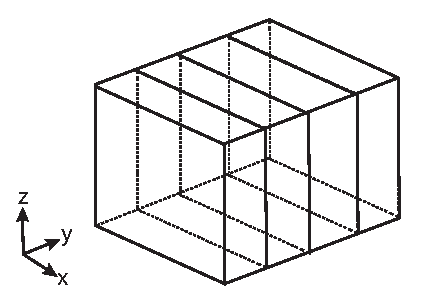
\includegraphics{Figures/2D_slices}
\decoRule
\caption[2D Sclices]{2D slices of the volume.}
\label{fig:2dslices}
\end{figure}
On modern graphics workstations, the complete process of interpolating texture coordinates and reconstructing texture values is incorporated into the scan-conversion process and done completely in hardware. Because texture mapping is such a common application, these routines are well-optimized and highly efficient.
To simulate ray casting using texture mapping, we have to slice the volumetric data set into parallel slices, and the use these slices as texture images to texture-map the projections of the sliced onto the image plane. To composite the slices, we can use the blending operations provided by the OpenGL graphics library. As it happens, one of the standard operators provided is exactly the compositing operator used in ray casting. Since compositing is also fully hardware-assisted, it is also very fast.
\begin{figure}[th]
\centering
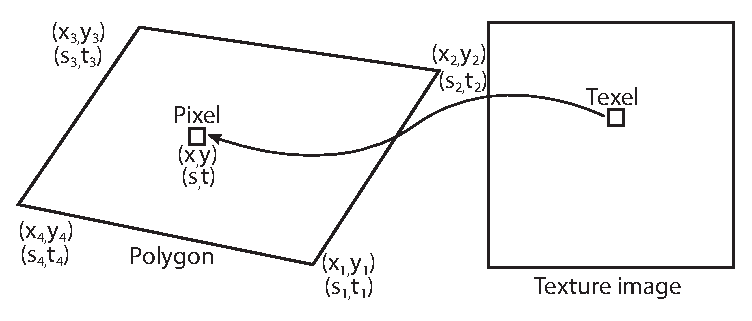
\includegraphics{Figures/2dtexmapping}
\decoRule
\caption[2D texture mapping]{Calculating color and opacity of a pixel inside a texture-mapped polygon.}
\label{fig:2dtexture}
\end{figure}

There are two ways to deal with varying viewpoints.

The first one is to create slice images for the given data set in a pre-processing step and uses different projection matrices to create arbitrary-viewpoint images of these slices. This is fast, since the (expensive) step of slice creation has to be done only once. On the other hand, image quality suffers because the views of all slices will be distorted due to the projection onto the image plane. In the extreme case of the view direction being parallel to the slices, there will be no image at all.

The second way is to create slices which are always orthogonal to the viewing direction. This results in optimal image quality, but it means that the slice stack has to be re-generated for each new image. Furthermore, arbitrary ("oblique") slices through a cuboid are generally not square or rectangular, and can be anything from triangles to hexagons.

\begin{algorithm} \caption{Volume Rendering using 2D Texture Mapping Algorithm} 
\label{alg:tex2dmapping}
\begin{algorithmic}[1]
\Require $N$ the number of slices, $\vec{v} $ the view direction
\State Load the data $\mathcal V(x,y,z) \gets data$ 
\State create the slices $s_i \in \mathcal V$ with each normal $\vec{n_i} \parallel \vec{v}$
\State Turn off the Depth test 
\State Enable the Blending 

\ForEach {$s_i \in \mathcal V $ form back to front}
\State $Texture \gets s_i$
\State create a polygon $p$ corresponding to the slice $s_i$
\State Assign texture coordinates to four corners of the polygon
\State Render and blend the polygon (alpha blending) 
\EndFor

\end{algorithmic}
\end{algorithm}

\paragraph{3D Texture mapping}
To allow interactive generation of view-orthogonal slices, a special hardware technique has been developed. This is a generalization of texture-mapping to three-dimensional textures, appropriately called "3D texturing."
As seen in Figure \ref{fig:2dtexture}, 2D texture-mapping interpolates two additional coordinates (s, t) across a polygon's interior. In 3D texture-mapping, three additional coordinates (s, t, r) are interpolated. To determine a pixel's color and opacity, these three coordinates are used as indices into a three-dimensional image, the 3D texture, see Figure \ref{fig:3dtexture}. To reconstruct texture values, tri-linear interpolation is used.

3D textures allow direct treatment of volumetric data. Instead of generating a set of two-dimensional slices in a pre-processing step, the volumetric data is directly downloaded into the graphics hardware, and is directly used to calculate color and opacity values for each pixel covered by a rendered primitive.

\begin{figure}[th]
\centering
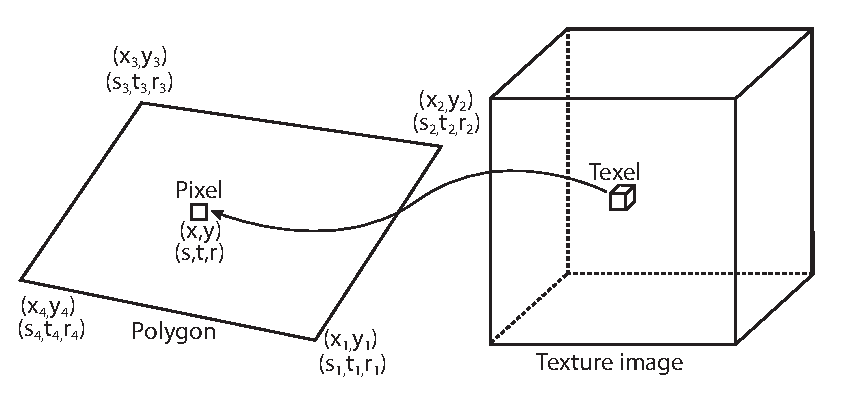
\includegraphics{Figures/3dtexmapping}
\decoRule
\caption[3D texture mapping]{Calculating color and opacity of a pixel inside a texture-mapped polygon using 3D texture.}
\label{fig:3dtexture}
\end{figure}


To generate oblique slices using 3D texturing, one only has to calculate the vertices of the slice, and then to generate the correct 3D texture coordinates for those vertices, see Figure \ref{fig:cubeSlice}. Then these coordinates are passed to the graphics library, and the graphics library will render the projection of the slice onto the image plane, using tri-linear interpolation to reconstruct each pixel's color and opacity values.

\begin{figure}[th]
\centering
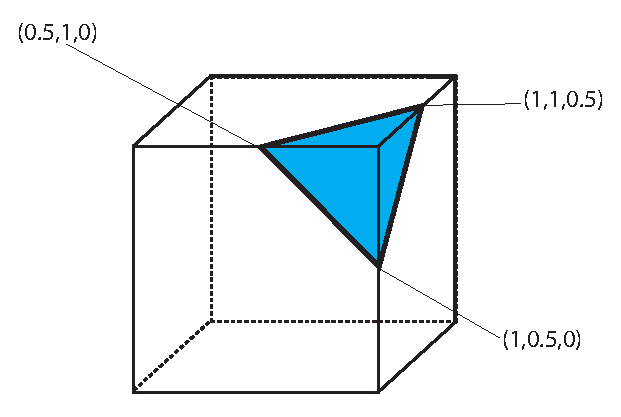
\includegraphics{Figures/cubeSlice}
\decoRule
\caption[3D Cube slice]{Calculating vertex coordinates and texture coordinates for an oblique slice. In this figure, the vertex and texture coordinates are identical.}
\label{fig:cubeSlice}
\end{figure}

\subsubsection{Raycasting}
Volume raycasting computes a 2D image from the 3D volumetric data set.The basic goal of ray casting is to allow the best use of the three-dimensional data and not attempt to impose any geometric structure on it. It solves one of the most important limitations of surface extraction techniques, namely the way in which they display a projection of a thin shell in the acquisition space. Surface extraction techniques fail to take into account that, particularly in medical imaging, data may originate from fluid and other materials which may be partially transparent and should be modeled as such. Ray casting doesn't suffer from this limitation. This algorithm can be split in four main steps (see Figure \ref{fig:rayasting}) :
\begin{itemize}

\item \textbf{Ray casting}. For each pixel of the final image, a ray of sight is shot ("cast") through the volume. At this stage it is useful to consider the volume being touched and enclosed within a bounding primitive, a simple geometric object (usually a cuboid) that is used to intersect the ray of sight and the volume.

\item \textbf{Sampling}. Along the part of the ray of sight that lies within the volume, equidistant sampling points or samples are selected. In general, the volume is not aligned with the ray of sight, and sampling points will usually be located in between voxels. Because of that, it is necessary to interpolate the values of the samples from its surrounding voxels (commonly using trilinear interpolation).

\item \textbf{Shading}. For each sampling point, a transfer function retrieves an RGBA material colour and a gradient of illumination values is computed. The gradient represents the orientation of local surfaces within the volume. The samples are then shaded (i.e. coloured and lit) according to their surface orientation and the location of the light source in the scene.

\item \textbf{Compositing}. After all sampling points have been shaded, they are composited along the ray of sight, resulting in the final colour value for the pixel that is currently being processed. The composition is derived directly from the rendering equation and is similar to blending acetate sheets on an overhead projector. It may work back-to-front, i.e. computation starts with the sample farthest from the viewer and ends with the one nearest to the viewer. This work flow direction ensures that masked parts of the volume do not affect the resulting pixel. The front-to-back order could be more computationally efficient since, the residual ray energy is getting down while ray travels away from camera; so, the contribution to the rendering integral is diminishing therefore more aggressive speed/quality compromise may be applied (increasing of distances between samples along ray is one of such speed/quality trade-offs).

\end{itemize}

\begin{figure}[th]
\centering
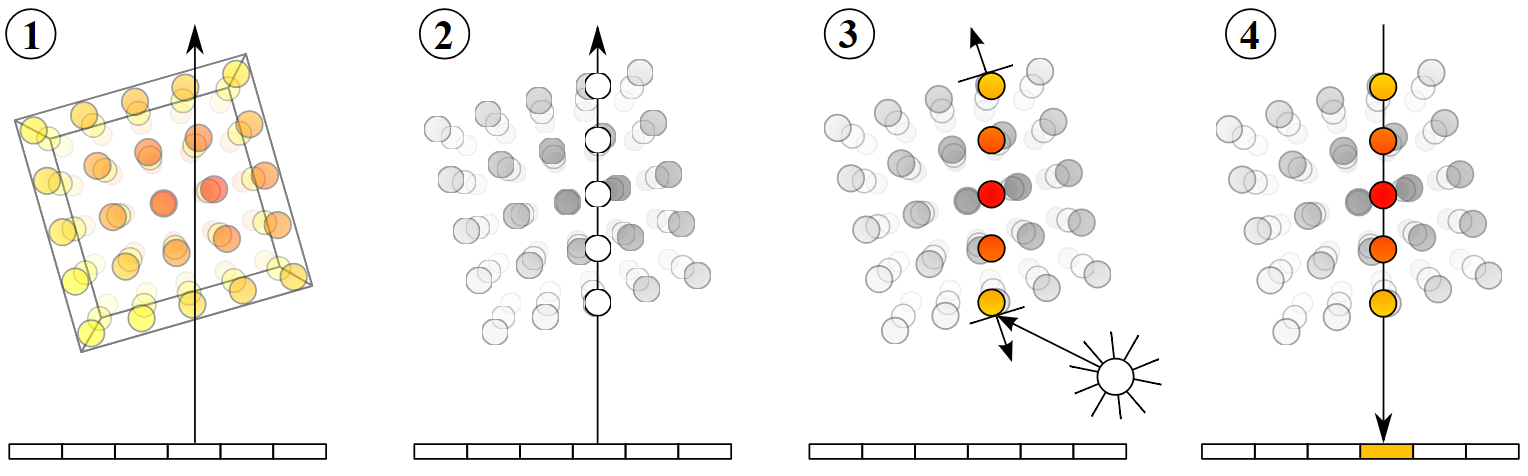
\includegraphics[width=\textwidth]{Figures/raycasting}
\decoRule
\caption[Volume raycasting]{ The four steps of the volume raycasting algorithm  }
\label{fig:rayasting}
\end{figure}

\subsection{Surface-fitting}


\section{Occlusion management strategies}



\subsection{Transfer Function}

A transfer function (TF) maps volumetric data to optical properties
and is part of the traditional visualization pipeline: data acquisition,
processing, visual mapping, and rendering. Volumetric data is
considered to be a scalar function from a three-dimensional spatial
domain with a one-dimensional range (e.g., density, flow magnitude,
etc.). Image generation involves mapping data samples through the
TF, where they are given optical properties such as color and opacity,
and compositing them into the image.
A TF simultaneously defines which parts of the data are essential
to depict and  how to depict these, often small, portions
of the volumetric data. Considering the first step, a TF is a special,
but important, case of a segmentation or classification. With classifi-
cation, certain regions in a three-dimensional domain are identified
to belong to the same material, such as bone, vessel, or soft tissue,
in medical imaging. A plethora of classification and segmentation
algorithms have been developed over the last decades, with semiautomatic
approaches often tailored to specific application scenarios.
Segmentation algorithms can be quite intricate since information
from the three-dimensional spatial domain and the one-dimensional
data range are taken into account. TFs in their basic form are, on the
other hand, restricted to using only the data ranges. In comparison
with general classification algorithms, this characteristic makes a
TF less powerful with respect to identifying relevant parts of the
data. The advantage of a TF is, however, a substantial performance
gain as classification based on the one-dimensional data range reduces
the complexity tremendously. This gain is the result of the
three-dimensional domain being typically two orders of magnitude
larger than the small data range. Histograms are an example of discarding
potentially complex spatial information and aggregating
only the data values to binned-frequency information. In the same
spirit, TFs classify interesting parts of the data by considering data
values alone. The second functionality of a TF deals with specifying
optical properties for portions of the data range previously identified
as being relevant

The transfer functions can be classified according to different criteria. Some of the most important are:

\begin{itemize}
\item \textbf{The dimension: } The one-dimensional TF classifies the scalar data value, $d$, and subsequently maps the material to an optical property for rendering: $ \textbf{q}(d)=\textbf{V}(\textbf{M}(d))$ where $\textbf{M}(.)$ is the material classification function and $\textbf{V}(.)$ is the
visual mapping of the material. One-dimensional TFs are adequate in many cases of simulation data where measurement noise is low or even non-existent where different materials of interest have few overlapping intensity
ranges \cite{4303986}. One-dimensional TFs are often the first tool available in software packages providing volume rendering, as they are relatively easy to comprehend for the novice or occasional user. Practically all production
visualization software, such as ParaView by \cite{paraview},
 VisIt by \cite{Childs:SciDAC2011}, 
or ImageVis3D by {\cite{Fogal2010Tuvok}}, support 1D TF editors.

\begin{figure}[th]
\centering
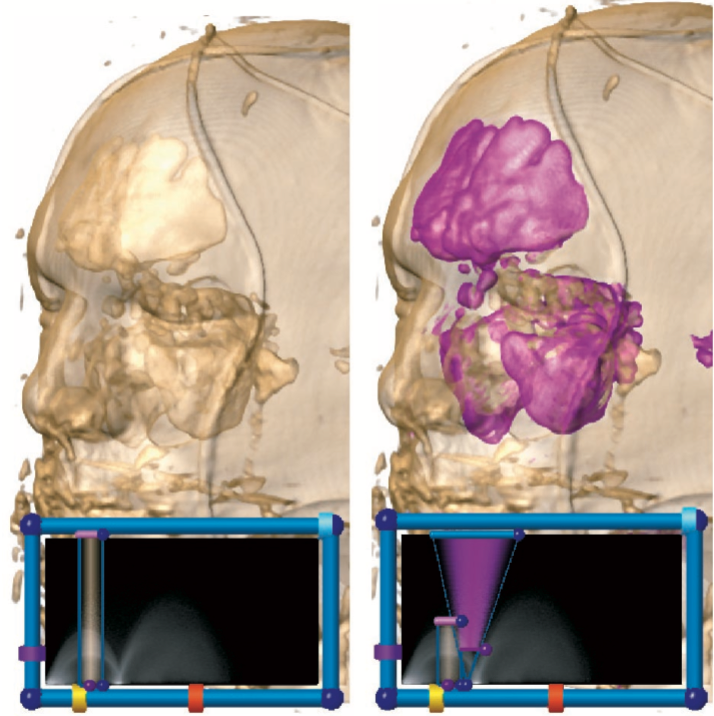
\includegraphics[width=\textwidth]{Figures/2dtf}
\decoRule
\caption[2D transfer Function]{ The two-dimensional TF editor widgets allow the user
to more precisely control the classification power of the 2D TF.
The triangular widget can also be skewed to better fit the desired
classification domain (\cite{1021579}) }
\label{fig:tf2d}
\end{figure}

Multidimensional TFs are used for Multidimensional data. If the user has to manipulate the TF definition directly, moving beyond
2D TFs immediately poses significant challenges in terms of
user interfaces and cognitive comprehension (\cite{1021579}). Much research and
work on Multidimensional TFs is, therefore, related to various forms of automation
and advanced user interfaces. Typical approaches include dimensional reduction, clustering
and grouping, machine learning, and various user interface
approaches such as parallel coordinates by \cite{5742368} or direct slice or volume
view interaction. 

\begin{figure}[th]
\centering
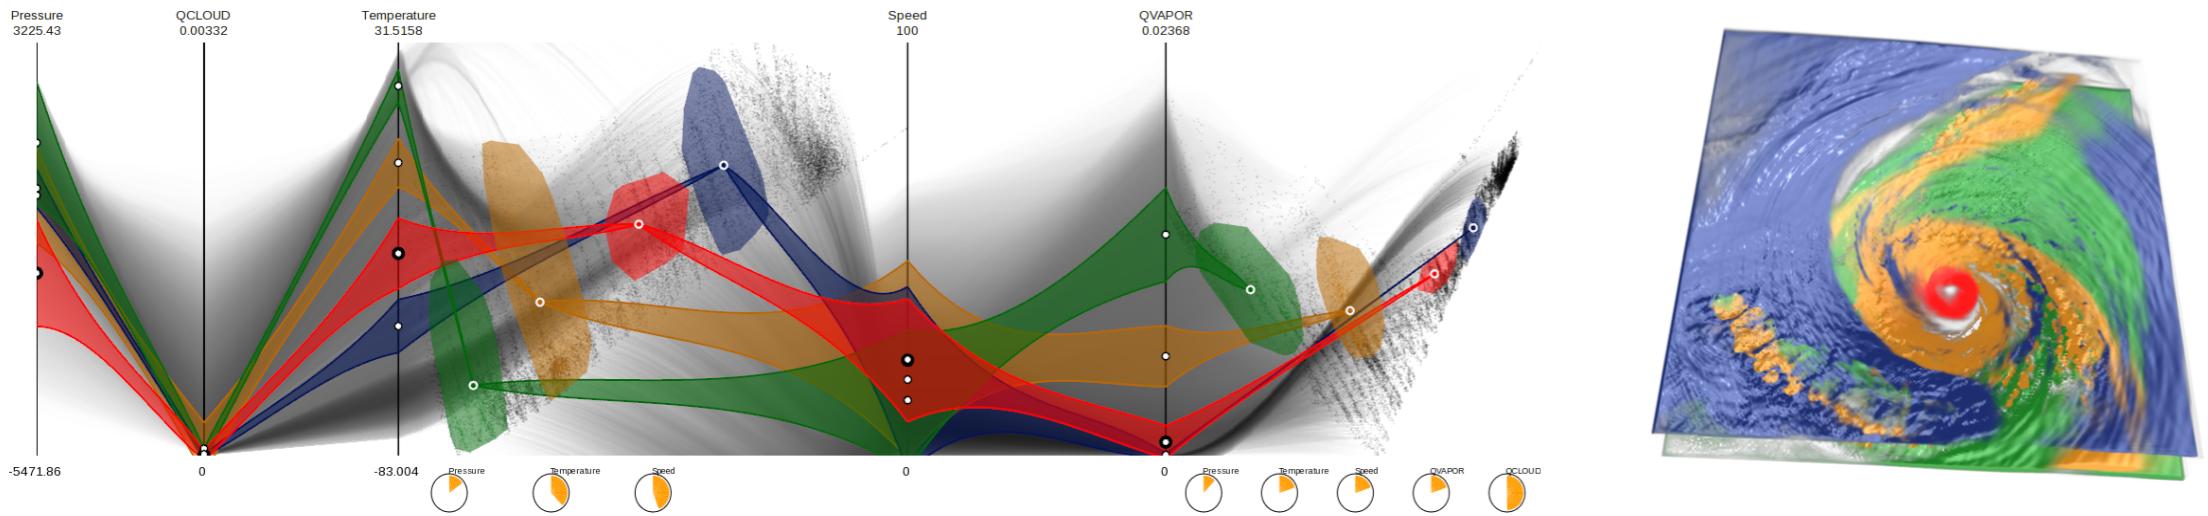
\includegraphics[width=\textwidth]{Figures/mdtf}
\decoRule
\caption[Multidimensional transfer Function]{ Parallel coordinates with embedded multidimensional scale plots for editing multidimensional TFs(\cite{5742368}) }
\label{fig:tfmd}
\end{figure}


\item \textbf{The automation}: The automation includes techniques such as adapting presets, semi-automatic, automatic, and supervised machine learning. Volume rendering has established itself as
a powerful visualization tool in many domains, but the necessary
design of TFs is a time consuming and tedious task. Consequently,
a significant amount of work is dedicated to the automatic and semiautomatic generation of TFs. 

\item \textbf{The aggregated attributes} : Conceptually, the introduction of additional quantities in the TF definition makes it possible to discriminate more parts in a dataset. Histogram clustering helps to reduce the degrees of freedom in designing a TF. As an illustration, \cite{5887324} propose modeling the
histogram space using a Gaussian mixture model. An elliptical TF
is assigned to each Gaussian, and the user interaction is simplified in order to edit the parameters of these ellipsoids.  

\end{itemize}

\subsection{Segmentation}

\subsection{Deformations and Focus + Context}

An interactive lens is a lightweight tool to solve a localized visualization problems by temporarily altering a selected part of the visual representation of the data~\cite{CGF:CGF12871}. Using this lens approach, we propose an interactive volume deformation based on GPU accelerated ray-casting to free a designated target from local occlusion while keeping the global context.

A lens is a parameterizable selection according to which a base visualization is altered. Typically, a lens is added to a visualization to interactively solve a specific localized problem. This property is very interesting with the aim of providing a focus+context solution to occlusion in volume rendering. Lenses can have different geometric properties not only defining their appearance, but also determining the selection, which is the subset of the data where these lenses take effect. The major geometric properties of a lens are shape, position, and size as well as the orientation.
The shape of a lens is usually chosen to fulfill the requirements of the application and is strongly linked to the lens function. Most virtual lenses are circular~\cite{1648236} or are rectangular~\cite{Kincaid:2010:SFA:1907651.1907963} as the real-world ones (magnifying glass, windows). Our lens has also a circular shape in order to remind its magnifying property. Some lenses, such as the  JellyLens~\cite{Pindat:2012:JCA:2380116.2380150} and the smart lenses~\cite{Thiede2008} can adapt their shape automatically according to the data. 
The position and the size parametrization can increase the flexibility of an interactive lens.
Modifying this position or size will set its focus on a different part of the data according to the user's interest. It is possible to update automatically these parameters in order to guide the user toward interesting events in the data~\cite{Tominski:2011:ECU:2336207.2336211}, or adjust the lens position according to predefined paths as the Routelens~\cite{Alvina:2014:RER:2598153.2598200} does. With this mind, our lens updates automatically its properties once a target has been selected. This allows a smooth transition towards an unobstructed and magnified area of interest. 

Lenses for volume visualization face challenges mainly related to spatial selection and occlusion. Wang et al. addressed these issues by proposing the Magic Lens~\cite{1532818}. This Magic Lens renders the obstructions with higher transparency and magnifies volumetric pre-computed features interactively or automatically in a pre-segmented dataset. In addition to interactively magnifying areas and objects of interest, our lens frees them from obstruction and allows local modification of the camera to see the target under other perspectives. Tong et al. proposed the GlyphLens~\cite{7539643} that removes the occluding glyphs by pulling the glyphs aside through the animation, but this tool is only well suited for systems where 3D volumetric dataset are visualized using glyphs. Lenses can create discontinuities between their inner part and the rest of the volume. Deformation can be a solution to this discontinuity issue.   




 \cite{Hsu:2011:RFM:2070781.2024165} developed a framework that can generate non-linear sampling rays that smoothly project objects in a scene at multiple levels of detail onto a single image. Such a technique requires a lot of computational time to render a single image from features of interest at different scales, see figure \ref{fig:multiscale}.This  multiscale rendering framework consists of a sequence of pinhole cameras, each of which captures a view of interest at a particular scale. The camera rays for each pixel in the final projected image are generated based on a user-defined image mask which specifies the interesting regions in each view.  The camera rays non-linearly cast through all scales of interest. Since the camera rays in the model are bent coherently and march consistently, the objects projected on the image are continuous in both image-space and object-space. 
 Their method starts by setting up several pinhole cameras for viewing different scales of interest, utilizing most users’ ease and familiarity with manipulating ordinary pinhole cameras. Each camera produces an image of its view. In order to combine all such views to form a single multiscale image, a user-specified image mask is used to indicate regions of each view that the user would like to show in the final image. In other words, every camera projects only part of its view onto the final image space, based on a corresponding image mask. In order to ensure consistency while projecting different camera
viewpoints onto different parts of the image, we force all camera rays to originate from the first camera, which is the one that has the largest scale of view. The rest of the cameras define intermediate
points that camera rays must pass through in order, from the largest to smallest scales. They use B\'ezier curves to connect the nearclipping planes of two successive cameras.

  The rays are bent gradually from one scale to another to maintain object-space continuity as well as image-space smoothness. The multiscale camera can also achieve a focus+context effect, a technique frequently used in many visualization applications. Finally, we show that it can potentially create pictures that mimic artistic or impossible views of objects or scenes like the kind made by the artist M. C. Escher. 
 
\begin{figure}[th]
\centering
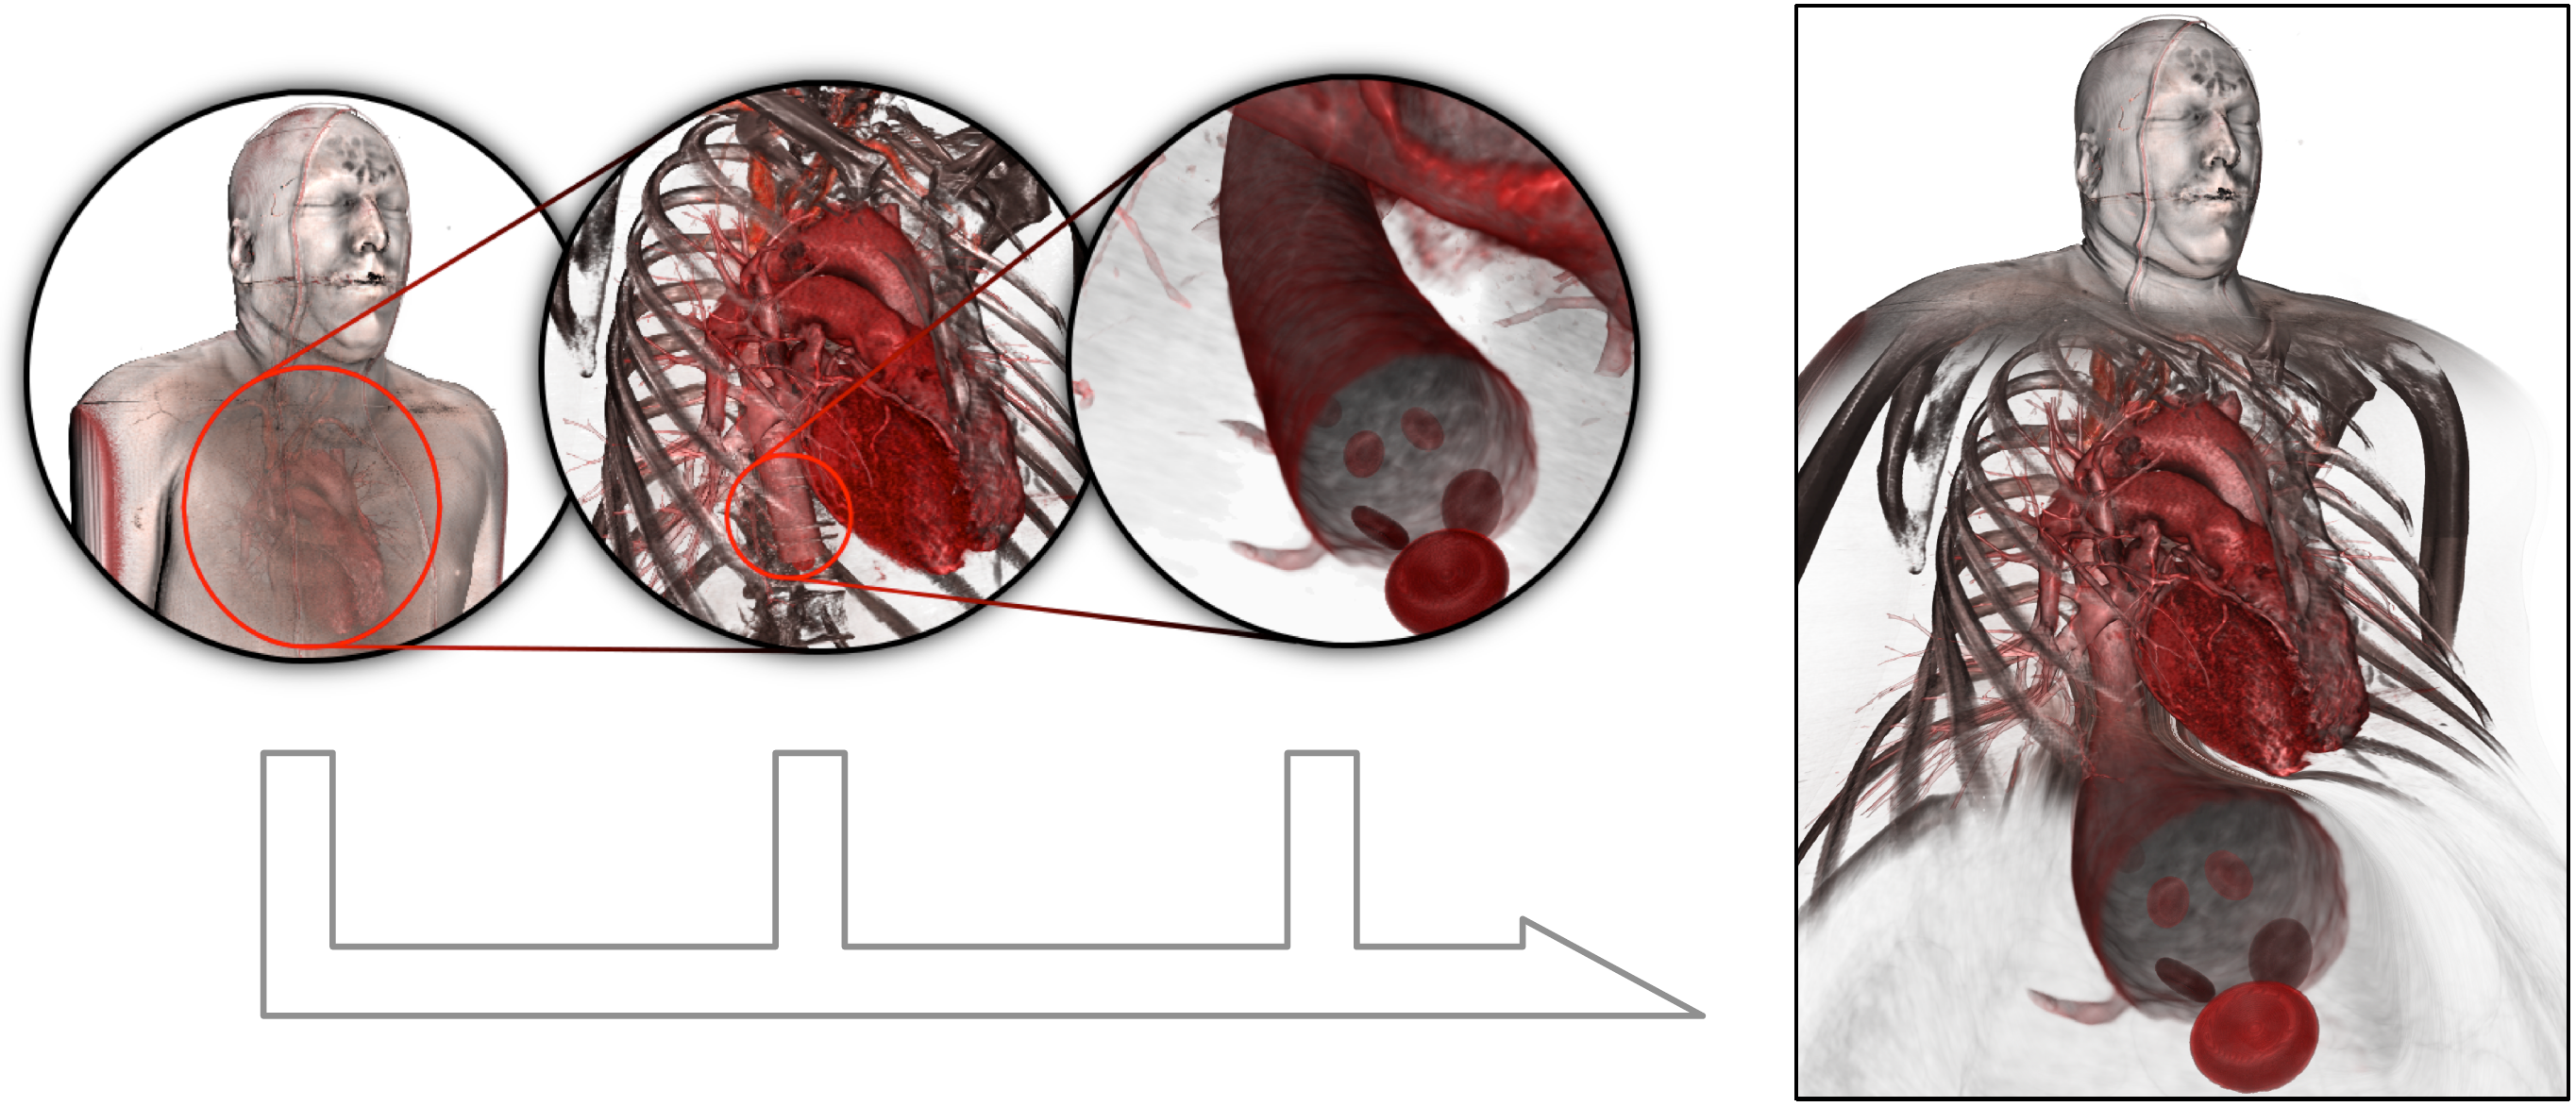
\includegraphics[width=\textwidth]{Figures/multiscale3d}
\decoRule
\caption[ multiscale ]{ A Rendering Framework for Multiscale Views of 3D Models. A continuous multiscale view (right) of a volumetric human body dataset shows three different levels of detail (left three) in a single image. The image on the right is directly rendered with our multiscale framework.}
\label{fig:multiscale}
\end{figure} 
 
  Bruckner and  Groller~\cite{4015467} proposed exploded view for volume data by partitioning the volume into several segments (figure \ref{fig:exploded}). Basically, in an exploded view the object is decomposed into several parts which are displaced so that internal details are visible. This does not only give an unobstructed view on the focus but also potentially reveals other interesting information, such as
cross-sections of the split object. The advantage of exploded views is that they simultaneously convey the global structure of the depicted object, the details of individual components, and the local relationships
among them. A Force-directed layout approach is used to arrange three-dimensional objects
in such a way that they do not occlude another object, but with as little displacement as possible. Four forces are used. \textbf{The Return force } is an attractive force that tries to move the parts towards
their original location. The force $F_r$ is realized as a logarithmic spring:
 \[ F_r=c_{r}\ln(||r||)\cdot \frac{r}{||r||} \] 
 where $r$ is the vector from the vertex's current position to its original location and $c_r$ is a constant factor.
 \textbf{The Explosion force} drives the specified parts away from our selection object. The explosion point is also weighted according to the size of the region corresponding to an octree node. Each explosion point exerts a force $F_e$ on every part $P_i$:
  \[ F_e=  \frac{c_e}{e^{||r||} } \cdot \frac{r}{||r||} \]
  where $r$ is the vector from the explosion point to the closest point of the part geometry of $P_i$ and $c_e$ is a scaling factor.
   \textbf{The Viewing force} is a view-dependent force which attempts to arrange parts so that they do not occlude the selection for the current viewing transformation. The force $F_v$ is:
   \[ F_v=  \frac{c_v}{||r||} \cdot \frac{r}{||r||} \] 
   where $r$ is the vector from the closest point along the viewing ray to the center of the body and $c_v$ is a scaling factor.
   \textbf{The Spacing force} prevents clustering of parts, we also add a
repulsive force $F_s$. For a part $P_i$, the spacing force exerted by another part $P_j$ is:
\[ F_s=  \frac{c_s}{||r||^2} \cdot \frac{r}{||r||} \] 
where $r$ is the vector from the center of $P_j$ to the center of $P_i$ and
$c_s$ is a constant scaling factor. 
\begin{figure}[th]
\centering
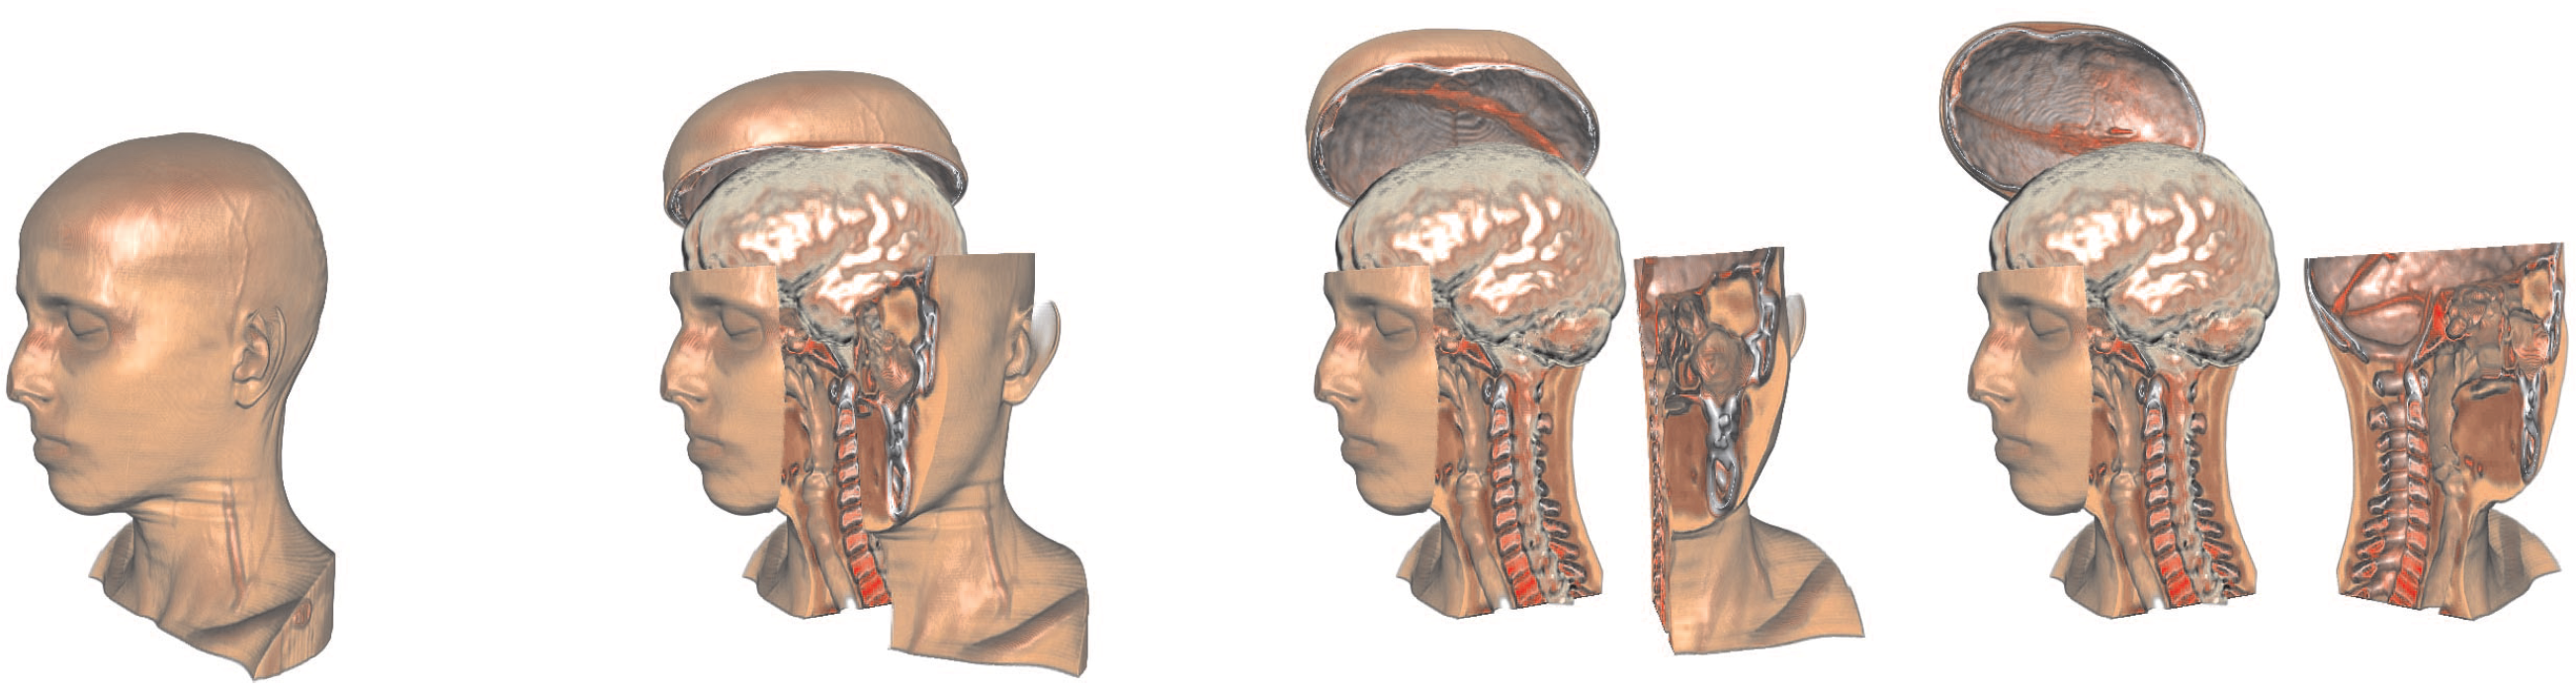
\includegraphics[width=\textwidth]{Figures/explodedview}
\decoRule
\caption[ Interactive exploded-view]{ Interactive exploded-view illustration of a human head with increasing degrees-of-explosion. Two hinge joints are used to constrain part
movement}
\label{fig:exploded}
\end{figure}
  
 
  
   McGuffin et al.~\cite{1250400} performed deformations using peeling to see hidden parts of the data. However, these techniques have the disadvantage of removing potentially important surrounding contextual information while trying to solve the local occlusion. 
 
 
Deformations can reveal predefined features in the dataset by taking into account the precomputed segmentation. Tong et al. proposed a deforming Lens which moves streamlines to observe the inner part of streamline bundles~\cite{7332955}. 


 Correa et al. proposed a framework~\cite{Correa:2007:IDD:1313046.1313163} allowing the users to physically or actively manipulate the geometry of a data object. Some studies performed deformations using surgical metaphors like ~\cite{4069230,Correa:2006:FAV:1187627.1187827} to see hidden parts of the volume, see figure \ref{fig:cut}. They propose a feature-based technique for manipulating volumetric objects for illustrative visualization, and describe a GPU-based implementation that enables interactive specification and their rendering.
Inspired by medical illustrations that frequently
depict the results of manipulation with tools such as peelers,
retractors and pliers, this system allows the specification of manipulation
through a collection of procedurally-defined manipulation operators.

\begin{figure}[th]
\centering
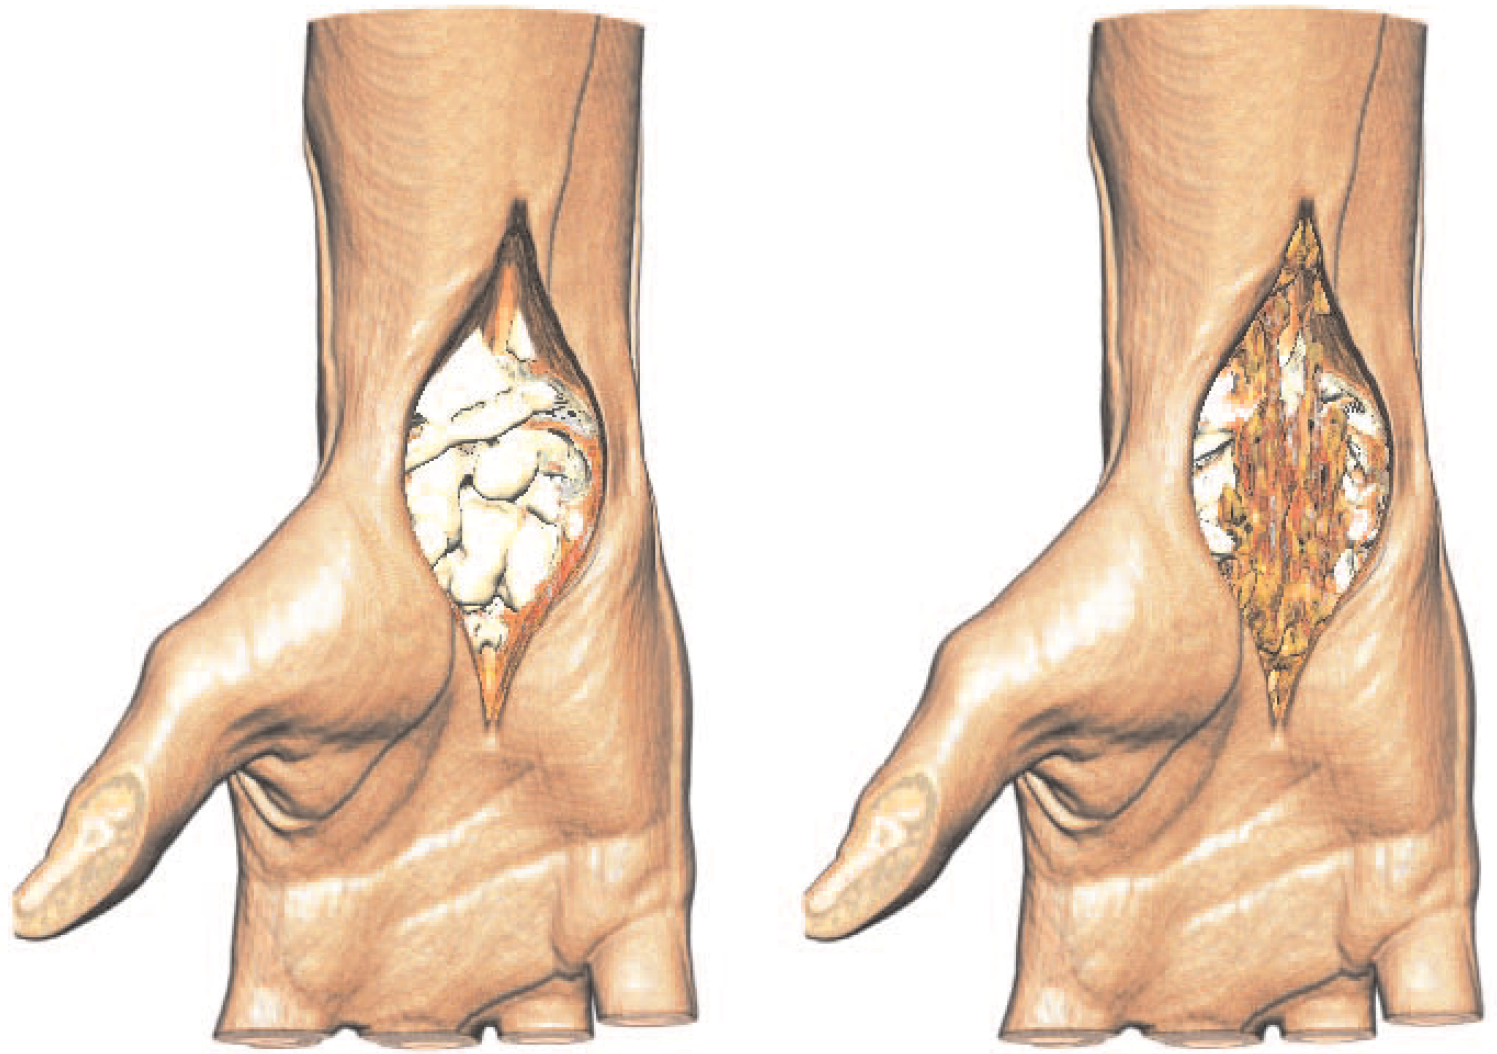
\includegraphics[width=\textwidth]{Figures/cut}
\decoRule
\caption[ Feature Aligned Volume Manipulation]{ A feature-aligned retraction applied to a human hand data set, showing bones (left) and vessels (right)}
\label{fig:cut}
\end{figure}

  \begin{figure}[th]
\centering
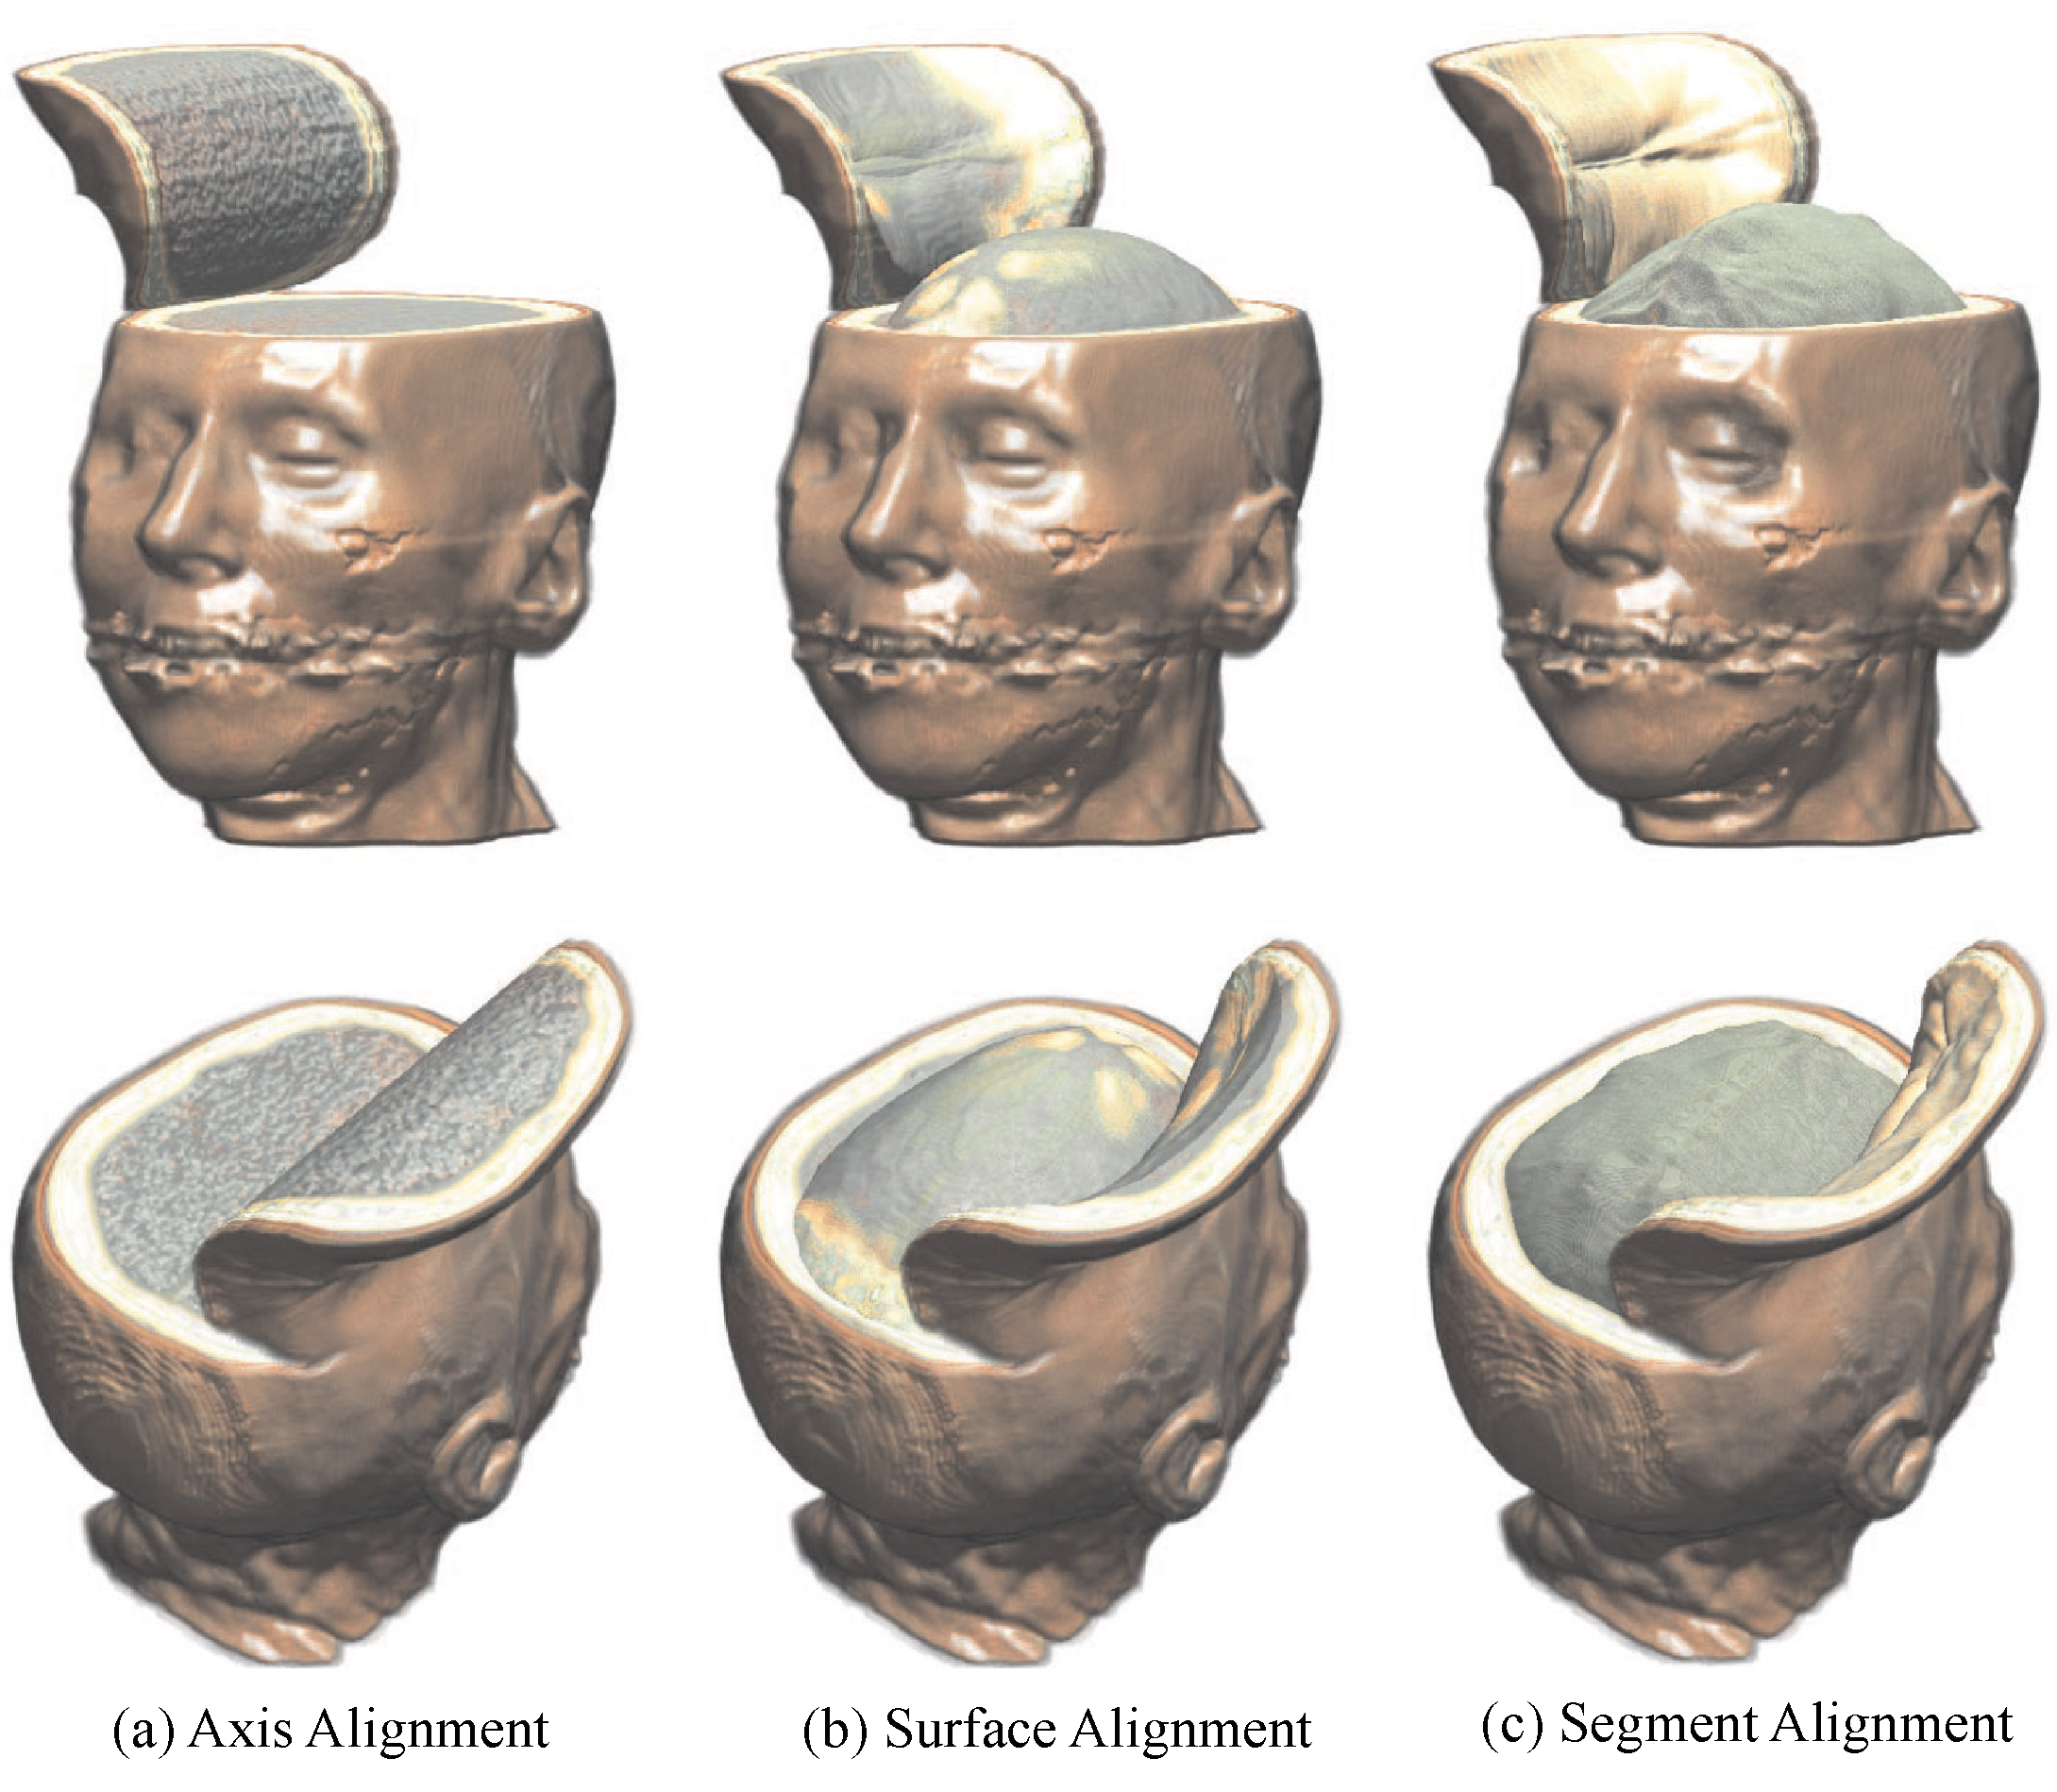
\includegraphics[width=\textwidth]{Figures/peel.pdf}
\decoRule
\caption[ Feature Aligned Volume Manipulation]{ An example of different types of alignment. (a) Axis aligned peel. Note how the peeled layer is thick and flat, since it is aligned with
an orthogonal axis. (b) Surface aligned peel, aligned with a computed
distance field. Notice how it approximates a surface. (c) Segment
aligned peel, based on segmentation, which is more accurate. Note
that in the feature based alignment (b) and (c) the peel is thin and
rounded.}
\label{fig:peel}
\end{figure}

 Correa et al. introduced two feature-based methods, namely surface alignment and segment alignment for modeling and rendering illustrative manipulation, and compare them with the traditional axis alignment method, see figure \ref{fig:peel}. They devise a method for estimating accurate normals along the surface of cuts
and dissections while maintaining continuous normals, which allows
us to obtain correct shading of the object being manipulated, opaque
or translucent. The four operators proposed in this framework are the following:
\begin{itemize}
\item Peeler: The peeler simulates peeling or cutting of the outer layers
of a volumetric model. Different parameters
of the peeler, such as thickness of the cut and the angle of bending of
the peeled layer, can be manipulated interactively to obtain different
illustrative effects.
\item Retractors: In the context of surgical illustration, retractors are tools used to spread organs or bones, or to hold back soft tissues such as
skin. In the context of illustration, they are useful for illustrating the
access to the internal organs.
\item Pliers: Pliers are tools used to grasp tissue and pull it or poke it into the volumetric object. The operator parameters include the shape of
the displacement and the radius of influence which specifies how the
displacement propagates through the volume.
\item Dilator: Dilators are used to gain access into narrow regions, cuts
or vessels. They essentially scale the region from the inside typically
by blowing air, to increase the visibility or accessibility of the region.
When applied to volumetric manipulation, dilators have a similar effect
to that of volumetric magic lenses (~\cite{1532818}).
\end{itemize} 
However this framework do not offer tools for local manipulation and exploration inside the cut, which allows perceiving a target under a different perspective while keeping the global context. 


\section{Volume rendering in Virtual Reality and Augmented Reality}

\subsection{ Remote volume rendering}

Volumetric data exploration with direct volume rendering technique is of great help to visually extract relevant structures in many fields of science: medical imaging ~\cite{ljung_full_2006}, astrophysics and more recently in baggage inspection. To leverage this knowledge extraction, many techniques have been developed. 

In this section, we detail existing ones with volume visualization, transfer function, direct voxel manipulation, and focus plus context interaction.
Volume visualization can be done with geometric rendering system which transforms the data into a set of polygons representing an iso-surface. The contour tree algorithm ~\cite{carr_computing_2000} and other alternatives such as branch decomposition ~\cite{pascucci_multi-resolution_2004} are usually used to find these iso-surfaces. According to H. Guo ~\cite{guo_local_2013}, contour trees algorithms are vulnerable to noises, which can be problematic in baggage inspections since dense materials (e.g. iron) cause noises by reflecting the X-rays. For this reason we used the volume rendering technique; Chen et al. provide a review of existing techniques ~\cite{chen_3-d_2000}.
In order to investigate volumetric dataset, one can use the Transfer Function (TF). In practice, it maps the voxel density with a specific color (including its transparency). Transfer function can be 1D, 2D or nD and are of great help to isolate structures of interest in volumetric data ~\cite{kniss_multidimensional_2002}. Thanks to the color blending process, suitable transfer function can also reveal iso surface or hide density to improve the volumetric data visualization. The setup of this transfer function remains complex, but some automatic systems provide solution thanks to data analysis ~\cite{correa_size-based_2008} ~\cite{sereda_visualization_2006} ~\cite{patel_moment_2009} or user interactions ~\cite{guo_wysiwyg_2011}. Since our users have a limited knowledge on volume rendering, we developed new interaction techniques with sufficient abstraction level regarding technical constraints. These techniques will be detailed in this paper. As an example, we investigated predefined transfer functions with smooth transitions when changing their setup to reduce disruptive animation effects ~\cite{tversky_animation:_2002}.
Since graphic card power never stops to improve, new techniques allow the direct manipulation of the voxels which composes the volume to be displayed. Color tunneling introduced a set of interactions (lock, Brush, Dig) to explore 2D and 3D dataset composed of pixels of voxels ~\cite{hurter_interactive_2014} with point based rendering techniques ~\cite{sainz_point-based_2004} . Histomage also provides direct manipulation of pixels thanks to a histogram which can be used as a new selection and pixel modification tool ~\cite{chevalier_histomages:_2012}. Other interactive systems investigated pixel exploration with a lens as a focus plus context technique ~\cite{elmqvist_color_2011} ~\cite{hurter_moleview:_2011}. Our work provides additional interaction techniques with pixel based techniques ~\cite{hurter_interactive_2014} to address occlusion issues, focus and context awareness, reversibility of the actions, and continuity.  
% Chapter 1

\chapter{Chapter Title Here} % Main chapter title

\label{Chapter1} % For referencing the chapter elsewhere, use \ref{Chapter1} 

%----------------------------------------------------------------------------------------

% Define some commands to keep the formatting separated from the content 
%\newcommand{\keyword}[1]{\textbf{#1}}
%\newcommand{\tabhead}[1]{\textbf{#1}}
%\newcommand{\code}[1]{\texttt{#1}}
%\newcommand{\file}[1]{\texttt{\bfseries#1}}
%\newcommand{\option}[1]{\texttt{\itshape#1}}

%----------------------------------------------------------------------------------------

\section{Welcome and Thank You}
Welcome to this \LaTeX{} Thesis Template, a beautiful and easy to use template for writing a thesis using the \LaTeX{} typesetting system.

If you are writing a thesis (or will be in the future) and its subject is technical or mathematical (though it doesn't have to be), then creating it in \LaTeX{} is highly recommended as a way to make sure you can just get down to the essential writing without having to worry over formatting or wasting time arguing with your word processor. 

\LaTeX{} is easily able to professionally typeset documents that run to hundreds or thousands of pages long. With simple mark-up commands, it automatically sets out the table of contents, margins, page headers and footers and keeps the formatting consistent and beautiful. One of its main strengths is the way it can easily typeset mathematics, even \emph{heavy} mathematics. Even if those equations are the most horribly twisted and most difficult mathematical problems that can only be solved on a super-computer, you can at least count on \LaTeX{} to make them look stunning.

%----------------------------------------------------------------------------------------

\section{Learning \LaTeX{}}

\LaTeX{} is not a \textsc{wysiwyg} (What You See is What You Get) program, unlike word processors such as Microsoft Word or Apple's Pages. Instead, a document written for \LaTeX{} is actually a simple, plain text file that contains \emph{no formatting}. You tell \LaTeX{} how you want the formatting in the finished document by writing in simple commands amongst the text, for example, if I want to use \emph{italic text for emphasis}, I write the \verb|\emph{text}| command and put the text I want in italics in between the curly braces. This means that \LaTeX{} is a \enquote{mark-up} language, very much like HTML.

\subsection{A (not so short) Introduction to \LaTeX{}}

If you are new to \LaTeX{}, there is a very good eBook -- freely available online as a PDF file -- called, \enquote{The Not So Short Introduction to \LaTeX{}}. The book's title is typically shortened to just \emph{lshort}. You can download the latest version (as it is occasionally updated) from here:
\url{http://www.ctan.org/tex-archive/info/lshort/english/lshort.pdf}

It is also available in several other languages. Find yours from the list on this page: \url{http://www.ctan.org/tex-archive/info/lshort/}

It is recommended to take a little time out to learn how to use \LaTeX{} by creating several, small `test' documents, or having a close look at several templates on:\\ 
\url{http://www.LaTeXTemplates.com}\\ 
Making the effort now means you're not stuck learning the system when what you \emph{really} need to be doing is writing your thesis.

\subsection{A Short Math Guide for \LaTeX{}}

If you are writing a technical or mathematical thesis, then you may want to read the document by the AMS (American Mathematical Society) called, \enquote{A Short Math Guide for \LaTeX{}}. It can be found online here:
\url{http://www.ams.org/tex/amslatex.html}
under the \enquote{Additional Documentation} section towards the bottom of the page.

\subsection{Common \LaTeX{} Math Symbols}
There are a multitude of mathematical symbols available for \LaTeX{} and it would take a great effort to learn the commands for them all. The most common ones you are likely to use are shown on this page:
\url{http://www.sunilpatel.co.uk/latex-type/latex-math-symbols/}

You can use this page as a reference or crib sheet, the symbols are rendered as large, high quality images so you can quickly find the \LaTeX{} command for the symbol you need.

\subsection{\LaTeX{} on a Mac}
 
The \LaTeX{} distribution is available for many systems including Windows, Linux and Mac OS X. The package for OS X is called MacTeX and it contains all the applications you need -- bundled together and pre-customized -- for a fully working \LaTeX{} environment and work flow.
 
MacTeX includes a custom dedicated \LaTeX{} editor called TeXShop for writing your `\file{.tex}' files and BibDesk: a program to manage your references and create your bibliography section just as easily as managing songs and creating playlists in iTunes.

%----------------------------------------------------------------------------------------

\section{Getting Started with this Template}

If you are familiar with \LaTeX{}, then you should explore the directory structure of the template and then proceed to place your own information into the \emph{THESIS INFORMATION} block of the \file{main.tex} file. You can then modify the rest of this file to your unique specifications based on your degree/university. Section \ref{FillingFile} on page \pageref{FillingFile} will help you do this. Make sure you also read section \ref{ThesisConventions} about thesis conventions to get the most out of this template.

If you are new to \LaTeX{} it is recommended that you carry on reading through the rest of the information in this document.

Before you begin using this template you should ensure that its style complies with the thesis style guidelines imposed by your institution. In most cases this template style and layout will be suitable. If it is not, it may only require a small change to bring the template in line with your institution's recommendations. These modifications will need to be done on the \file{MastersDoctoralThesis.cls} file.

\subsection{About this Template}

This \LaTeX{} Thesis Template is originally based and created around a \LaTeX{} style file created by Steve R.\ Gunn from the University of Southampton (UK), department of Electronics and Computer Science. You can find his original thesis style file at his site, here:
\url{http://www.ecs.soton.ac.uk/~srg/softwaretools/document/templates/}

Steve's \file{ecsthesis.cls} was then taken by Sunil Patel who modified it by creating a skeleton framework and folder structure to place the thesis files in. The resulting template can be found on Sunil's site here:
\url{http://www.sunilpatel.co.uk/thesis-template}

Sunil's template was made available through \url{http://www.LaTeXTemplates.com} where it was modified many times based on user requests and questions. Version 2.0 and onwards of this template represents a major modification to Sunil's template and is, in fact, hardly recognisable. The work to make version 2.0 possible was carried out by \href{mailto:vel@latextemplates.com}{Vel} and Johannes Böttcher.

%----------------------------------------------------------------------------------------

\section{What this Template Includes}

\subsection{Folders}

This template comes as a single zip file that expands out to several files and folders. The folder names are mostly self-explanatory:

\keyword{Appendices} -- this is the folder where you put the appendices. Each appendix should go into its own separate \file{.tex} file. An example and template are included in the directory.

\keyword{Chapters} -- this is the folder where you put the thesis chapters. A thesis usually has about six chapters, though there is no hard rule on this. Each chapter should go in its own separate \file{.tex} file and they can be split as:
\begin{itemize}
\item Chapter 1: Introduction to the thesis topic
\item Chapter 2: Background information and theory
\item Chapter 3: (Laboratory) experimental setup
\item Chapter 4: Details of experiment 1
\item Chapter 5: Details of experiment 2
\item Chapter 6: Discussion of the experimental results
\item Chapter 7: Conclusion and future directions
\end{itemize}
This chapter layout is specialised for the experimental sciences, your discipline may be different.

\keyword{Figures} -- this folder contains all figures for the thesis. These are the final images that will go into the thesis document.

\subsection{Files}

Included are also several files, most of them are plain text and you can see their contents in a text editor. After initial compilation, you will see that more auxiliary files are created by \LaTeX{} or BibTeX and which you don't need to delete or worry about:

\keyword{example.bib} -- this is an important file that contains all the bibliographic information and references that you will be citing in the thesis for use with BibTeX. You can write it manually, but there are reference manager programs available that will create and manage it for you. Bibliographies in \LaTeX{} are a large subject and you may need to read about BibTeX before starting with this. Many modern reference managers will allow you to export your references in BibTeX format which greatly eases the amount of work you have to do.

\keyword{MastersDoctoralThesis.cls} -- this is an important file. It is the class file that tells \LaTeX{} how to format the thesis. 

\keyword{main.pdf} -- this is your beautifully typeset thesis (in the PDF file format) created by \LaTeX{}. It is supplied in the PDF with the template and after you compile the template you should get an identical version.

\keyword{main.tex} -- this is an important file. This is the file that you tell \LaTeX{} to compile to produce your thesis as a PDF file. It contains the framework and constructs that tell \LaTeX{} how to layout the thesis. It is heavily commented so you can read exactly what each line of code does and why it is there. After you put your own information into the \emph{THESIS INFORMATION} block -- you have now started your thesis!

Files that are \emph{not} included, but are created by \LaTeX{} as auxiliary files include:

\keyword{main.aux} -- this is an auxiliary file generated by \LaTeX{}, if it is deleted \LaTeX{} simply regenerates it when you run the main \file{.tex} file.

\keyword{main.bbl} -- this is an auxiliary file generated by BibTeX, if it is deleted, BibTeX simply regenerates it when you run the \file{main.aux} file. Whereas the \file{.bib} file contains all the references you have, this \file{.bbl} file contains the references you have actually cited in the thesis and is used to build the bibliography section of the thesis.

\keyword{main.blg} -- this is an auxiliary file generated by BibTeX, if it is deleted BibTeX simply regenerates it when you run the main \file{.aux} file.

\keyword{main.lof} -- this is an auxiliary file generated by \LaTeX{}, if it is deleted \LaTeX{} simply regenerates it when you run the main \file{.tex} file. It tells \LaTeX{} how to build the \emph{List of Figures} section.

\keyword{main.log} -- this is an auxiliary file generated by \LaTeX{}, if it is deleted \LaTeX{} simply regenerates it when you run the main \file{.tex} file. It contains messages from \LaTeX{}, if you receive errors and warnings from \LaTeX{}, they will be in this \file{.log} file.

\keyword{main.lot} -- this is an auxiliary file generated by \LaTeX{}, if it is deleted \LaTeX{} simply regenerates it when you run the main \file{.tex} file. It tells \LaTeX{} how to build the \emph{List of Tables} section.

\keyword{main.out} -- this is an auxiliary file generated by \LaTeX{}, if it is deleted \LaTeX{} simply regenerates it when you run the main \file{.tex} file.

So from this long list, only the files with the \file{.bib}, \file{.cls} and \file{.tex} extensions are the most important ones. The other auxiliary files can be ignored or deleted as \LaTeX{} and BibTeX will regenerate them.

%----------------------------------------------------------------------------------------

\section{Filling in Your Information in the \file{main.tex} File}\label{FillingFile}

You will need to personalise the thesis template and make it your own by filling in your own information. This is done by editing the \file{main.tex} file in a text editor or your favourite LaTeX environment.

Open the file and scroll down to the third large block titled \emph{THESIS INFORMATION} where you can see the entries for \emph{University Name}, \emph{Department Name}, etc \ldots

Fill out the information about yourself, your group and institution. You can also insert web links, if you do, make sure you use the full URL, including the \code{http://} for this. If you don't want these to be linked, simply remove the \verb|\href{url}{name}| and only leave the name.

When you have done this, save the file and recompile \code{main.tex}. All the information you filled in should now be in the PDF, complete with web links. You can now begin your thesis proper!

%----------------------------------------------------------------------------------------

\section{The \code{main.tex} File Explained}

The \file{main.tex} file contains the structure of the thesis. There are plenty of written comments that explain what pages, sections and formatting the \LaTeX{} code is creating. Each major document element is divided into commented blocks with titles in all capitals to make it obvious what the following bit of code is doing. Initially there seems to be a lot of \LaTeX{} code, but this is all formatting, and it has all been taken care of so you don't have to do it.

Begin by checking that your information on the title page is correct. For the thesis declaration, your institution may insist on something different than the text given. If this is the case, just replace what you see with what is required in the \emph{DECLARATION PAGE} block.

Then comes a page which contains a funny quote. You can put your own, or quote your favourite scientist, author, person, and so on. Make sure to put the name of the person who you took the quote from.

Following this is the abstract page which summarises your work in a condensed way and can almost be used as a standalone document to describe what you have done. The text you write will cause the heading to move up so don't worry about running out of space.

Next come the acknowledgements. On this page, write about all the people who you wish to thank (not forgetting parents, partners and your advisor/supervisor).

The contents pages, list of figures and tables are all taken care of for you and do not need to be manually created or edited. The next set of pages are more likely to be optional and can be deleted since they are for a more technical thesis: insert a list of abbreviations you have used in the thesis, then a list of the physical constants and numbers you refer to and finally, a list of mathematical symbols used in any formulae. Making the effort to fill these tables means the reader has a one-stop place to refer to instead of searching the internet and references to try and find out what you meant by certain abbreviations or symbols.

The list of symbols is split into the Roman and Greek alphabets. Whereas the abbreviations and symbols ought to be listed in alphabetical order (and this is \emph{not} done automatically for you) the list of physical constants should be grouped into similar themes.

The next page contains a one line dedication. Who will you dedicate your thesis to?

Finally, there is the block where the chapters are included. Uncomment the lines (delete the \code{\%} character) as you write the chapters. Each chapter should be written in its own file and put into the \emph{Chapters} folder and named \file{Chapter1}, \file{Chapter2}, etc\ldots Similarly for the appendices, uncomment the lines as you need them. Each appendix should go into its own file and placed in the \emph{Appendices} folder.

After the preamble, chapters and appendices finally comes the bibliography. The bibliography style (called \option{authoryear}) is used for the bibliography and is a fully featured style that will even include links to where the referenced paper can be found online. Do not underestimate how grateful your reader will be to find that a reference to a paper is just a click away. Of course, this relies on you putting the URL information into the BibTeX file in the first place.

%----------------------------------------------------------------------------------------

\section{Thesis Features and Conventions}\label{ThesisConventions}

To get the best out of this template, there are a few conventions that you may want to follow.

One of the most important (and most difficult) things to keep track of in such a long document as a thesis is consistency. Using certain conventions and ways of doing things (such as using a Todo list) makes the job easier. Of course, all of these are optional and you can adopt your own method.

\subsection{Printing Format}

This thesis template is designed for double sided printing (i.e. content on the front and back of pages) as most theses are printed and bound this way. Switching to one sided printing is as simple as uncommenting the \option{oneside} option of the \code{documentclass} command at the top of the \file{main.tex} file. You may then wish to adjust the margins to suit specifications from your institution.

The headers for the pages contain the page number on the outer side (so it is easy to flick through to the page you want) and the chapter name on the inner side.

The text is set to 11 point by default with single line spacing, again, you can tune the text size and spacing should you want or need to using the options at the very start of \file{main.tex}. The spacing can be changed similarly by replacing the \option{singlespacing} with \option{onehalfspacing} or \option{doublespacing}.

\subsection{Using US Letter Paper}

The paper size used in the template is A4, which is the standard size in Europe. If you are using this thesis template elsewhere and particularly in the United States, then you may have to change the A4 paper size to the US Letter size. This can be done in the margins settings section in \file{main.tex}.

Due to the differences in the paper size, the resulting margins may be different to what you like or require (as it is common for institutions to dictate certain margin sizes). If this is the case, then the margin sizes can be tweaked by modifying the values in the same block as where you set the paper size. Now your document should be set up for US Letter paper size with suitable margins.

\subsection{References}

The \code{biblatex} package is used to format the bibliography and inserts references such as this one \parencite{Reference1}. The options used in the \file{main.tex} file mean that the in-text citations of references are formatted with the author(s) listed with the date of the publication. Multiple references are separated by semicolons (e.g. \parencite{Reference2, Reference1}) and references with more than three authors only show the first author with \emph{et al.} indicating there are more authors (e.g. \parencite{Reference3}). This is done automatically for you. To see how you use references, have a look at the \file{Chapter1.tex} source file. Many reference managers allow you to simply drag the reference into the document as you type.

Scientific references should come \emph{before} the punctuation mark if there is one (such as a comma or period). The same goes for footnotes\footnote{Such as this footnote, here down at the bottom of the page.}. You can change this but the most important thing is to keep the convention consistent throughout the thesis. Footnotes themselves should be full, descriptive sentences (beginning with a capital letter and ending with a full stop). The APA6 states: \enquote{Footnote numbers should be superscripted, [...], following any punctuation mark except a dash.} The Chicago manual of style states: \enquote{A note number should be placed at the end of a sentence or clause. The number follows any punctuation mark except the dash, which it precedes. It follows a closing parenthesis.}

The bibliography is typeset with references listed in alphabetical order by the first author's last name. This is similar to the APA referencing style. To see how \LaTeX{} typesets the bibliography, have a look at the very end of this document (or just click on the reference number links in in-text citations).

\subsubsection{A Note on bibtex}

The bibtex backend used in the template by default does not correctly handle unicode character encoding (i.e. "international" characters). You may see a warning about this in the compilation log and, if your references contain unicode characters, they may not show up correctly or at all. The solution to this is to use the biber backend instead of the outdated bibtex backend. This is done by finding this in \file{main.tex}: \option{backend=bibtex} and changing it to \option{backend=biber}. You will then need to delete all auxiliary BibTeX files and navigate to the template directory in your terminal (command prompt). Once there, simply type \code{biber main} and biber will compile your bibliography. You can then compile \file{main.tex} as normal and your bibliography will be updated. An alternative is to set up your LaTeX editor to compile with biber instead of bibtex, see \href{http://tex.stackexchange.com/questions/154751/biblatex-with-biber-configuring-my-editor-to-avoid-undefined-citations/}{here} for how to do this for various editors.

\subsection{Tables}

Tables are an important way of displaying your results, below is an example table which was generated with this code:

{\small
\begin{verbatim}
\begin{table}
\caption{The effects of treatments X and Y on the four groups studied.}
\label{tab:treatments}
\centering
\begin{tabular}{l l l}
\toprule
\tabhead{Groups} & \tabhead{Treatment X} & \tabhead{Treatment Y} \\
\midrule
1 & 0.2 & 0.8\\
2 & 0.17 & 0.7\\
3 & 0.24 & 0.75\\
4 & 0.68 & 0.3\\
\bottomrule\\
\end{tabular}
\end{table}
\end{verbatim}
}

\begin{table}
\caption{The effects of treatments X and Y on the four groups studied.}
\label{tab:treatments}
\centering
\begin{tabular}{l l l}
\toprule
\tabhead{Groups} & \tabhead{Treatment X} & \tabhead{Treatment Y} \\
\midrule
1 & 0.2 & 0.8\\
2 & 0.17 & 0.7\\
3 & 0.24 & 0.75\\
4 & 0.68 & 0.3\\
\bottomrule\\
\end{tabular}
\end{table}

You can reference tables with \verb|\ref{<label>}| where the label is defined within the table environment. See \file{Chapter1.tex} for an example of the label and citation (e.g. Table~\ref{tab:treatments}).

\subsection{Figures}

There will hopefully be many figures in your thesis (that should be placed in the \emph{Figures} folder). The way to insert figures into your thesis is to use a code template like this:
\begin{verbatim}
\begin{figure}
\centering

\includegraphics{Figures/Electron}
\decoRule
\caption[An Electron]{An electron (artist's impression).}
\label{fig:Electron}
\end{figure}
\end{verbatim}
Also look in the source file. Putting this code into the source file produces the picture of the electron that you can see in the figure below.

\begin{figure}[th]
\centering

\includegraphics{Figures/Electron}
\decoRule
\caption[An Electron]{An electron (artist's impression).}
\label{fig:Electron}
\end{figure}

Sometimes figures don't always appear where you write them in the source. The placement depends on how much space there is on the page for the figure. Sometimes there is not enough room to fit a figure directly where it should go (in relation to the text) and so \LaTeX{} puts it at the top of the next page. Positioning figures is the job of \LaTeX{} and so you should only worry about making them look good!

Figures usually should have captions just in case you need to refer to them (such as in Figure~\ref{fig:Electron}). The \verb|\caption| command contains two parts, the first part, inside the square brackets is the title that will appear in the \emph{List of Figures}, and so should be short. The second part in the curly brackets should contain the longer and more descriptive caption text.

The \verb|\decoRule| command is optional and simply puts an aesthetic horizontal line below the image. If you do this for one image, do it for all of them.

\LaTeX{} is capable of using images in pdf, jpg and png format.

\subsection{Typesetting mathematics}

If your thesis is going to contain heavy mathematical content, be sure that \LaTeX{} will make it look beautiful, even though it won't be able to solve the equations for you.

The \enquote{Not So Short Introduction to \LaTeX} (available on \href{http://www.ctan.org/tex-archive/info/lshort/english/lshort.pdf}{CTAN}) should tell you everything you need to know for most cases of typesetting mathematics. If you need more information, a much more thorough mathematical guide is available from the AMS called, \enquote{A Short Math Guide to \LaTeX} and can be downloaded from:
\url{ftp://ftp.ams.org/pub/tex/doc/amsmath/short-math-guide.pdf}

There are many different \LaTeX{} symbols to remember, luckily you can find the most common symbols in \href{http://ctan.org/pkg/comprehensive}{The Comprehensive \LaTeX~Symbol List}.

You can write an equation, which is automatically given an equation number by \LaTeX{} like this:
\begin{verbatim}
\begin{equation}
E = mc^{2}
\label{eqn:Einstein}
\end{equation}
\end{verbatim}

This will produce Einstein's famous energy-matter equivalence equation:
\begin{equation}
E = mc^{2}
\label{eqn:Einstein}
\end{equation}

All equations you write (which are not in the middle of paragraph text) are automatically given equation numbers by \LaTeX{}. If you don't want a particular equation numbered, use the unnumbered form:
\begin{verbatim}
\[ a^{2}=4 \]
\end{verbatim}

%----------------------------------------------------------------------------------------

\section{Sectioning and Subsectioning}

You should break your thesis up into nice, bite-sized sections and subsections. \LaTeX{} automatically builds a table of Contents by looking at all the \verb|\chapter{}|, \verb|\section{}|  and \verb|\subsection{}| commands you write in the source.

The Table of Contents should only list the sections to three (3) levels. A \verb|chapter{}| is level zero (0). A \verb|\section{}| is level one (1) and so a \verb|\subsection{}| is level two (2). In your thesis it is likely that you will even use a \verb|subsubsection{}|, which is level three (3). The depth to which the Table of Contents is formatted is set within \file{MastersDoctoralThesis.cls}. If you need this changed, you can do it in \file{main.tex}.

%----------------------------------------------------------------------------------------

\section{In Closing}

You have reached the end of this mini-guide. You can now rename or overwrite this pdf file and begin writing your own \file{Chapter1.tex} and the rest of your thesis. The easy work of setting up the structure and framework has been taken care of for you. It's now your job to fill it out!

Good luck and have lots of fun!

\begin{flushright}
Guide written by ---\\
Sunil Patel: \href{http://www.sunilpatel.co.uk}{www.sunilpatel.co.uk}\\
Vel: \href{http://www.LaTeXTemplates.com}{LaTeXTemplates.com}
\end{flushright}


%\include{Chapters/Chapter2} 
%\include{Chapters/Chapter3}
%\include{Chapters/Chapter4} 
%\include{Chapters/Chapter5} 

%----------------------------------------------------------------------------------------
%	THESIS CONTENT - APPENDICES
%----------------------------------------------------------------------------------------

\appendix % Cue to tell LaTeX that the following "chapters" are Appendices

% Include the appendices of the thesis as separate files from the Appendices folder
% Uncomment the lines as you write the Appendices

% Appendix A

\chapter{Frequently Asked Questions} % Main appendix title

\label{AppendixA} % For referencing this appendix elsewhere, use \ref{AppendixA}

\section{How do I change the colors of links?}

The color of links can be changed to your liking using:

{\small\verb!\hypersetup{urlcolor=red}!}, or

{\small\verb!\hypersetup{citecolor=green}!}, or

{\small\verb!\hypersetup{allcolor=blue}!}.

\noindent If you want to completely hide the links, you can use:

{\small\verb!\hypersetup{allcolors=.}!}, or even better: 

{\small\verb!\hypersetup{hidelinks}!}.

\noindent If you want to have obvious links in the PDF but not the printed text, use:

{\small\verb!\hypersetup{colorlinks=false}!}.

%\include{Appendices/AppendixB}
%\include{Appendices/AppendixC}

%----------------------------------------------------------------------------------------
%	BIBLIOGRAPHY
%----------------------------------------------------------------------------------------

\printbibliography[heading=bibintoc]

%----------------------------------------------------------------------------------------

\end{document}  
